\documentclass[a4paper,11pt,oneside]{book}
\usepackage[utf8]{inputenc}
\usepackage[english,italian]{babel}
\usepackage{geometry}
\usepackage{fancyhdr}
\usepackage{makeidx}
\usepackage{graphicx}
\usepackage{subcaption}
\usepackage{xfrac}
\usepackage{float}
\usepackage{tocloft}
\usepackage{nomencl}
\usepackage[T1]{fontenc}
\usepackage{tikz-cd}
\usepackage[pdfa, hidelinks]{hyperref}
\usepackage{hyperxmp}
\usepackage{embedfile}
\usepackage{multirow}
\usepackage{epigraph}
\usepackage{tocbibind}
\usepackage{amsmath, amsthm, amssymb, amsfonts}
\usepackage{thmtools}
\usepackage{setspace}
\usepackage{framed}
\graphicspath{./figs/}
\title{Definition of the lithospheric structure of the Ionian basin.}
\author{Francesco De Rose, Mario La Rocca, Luca De Siena}
\date{October 2025}
\hypersetup{%
pdflang=la,
pdfapart=3,
pdfaconformance=B
}
\geometry{
    top=2.6cm,
    bottom=2.6cm,
    left=3.2cm,
    right=3.2cm,
}
\setlength{\parindent}{0cm}
\setlength{\marginparwidth}{3cm}
\setlength{\headheight}{18pt}
\linespread{1.1}
\pagestyle{fancy}
\fancyhf{}
\rhead{\leftmark}
\cfoot{\thepage}
\def\blankpage{
      \clearpage
      \thispagestyle{empty}
      \null%
      \clearpage}     
\newenvironment{dedication}
  {\thispagestyle{empty}
   \vspace*{\stretch{1}}
   \itshape             
   \raggedleft}
  {\par 
   \vspace{\stretch{3}} 
   \clearpage}
\begin{document}
\begin{titlepage}
    \begin{center}
\textbf{\LARGE University of Calabria}\\
        \textbf{Physics department}\\
        \vskip 6pt
        \hrule
        \vskip 8pt
        \includegraphics{./figs/unical.png}
        \vskip 8pt
        \textbf{Master’s Degree  in  Physics}
        \vskip 32pt
            
            \large{Thesis}


        \vskip 70pt
        {  
            \huge \bfseries Definition of the lithospheric structure of the Ionian basin.
        }
        \\[0.4cm]

        \vskip 80pt

        \begin{tabular}{p{8cm}p{8cm}}
            Supervisors:     & Candidate:\\
            Prof.  Mario La Rocca      & Francesco De Rose \\
            Prof. Luca De Siena & Serial number 256865 \\
            Thesis supervisor:\\
            Prof. Fabio Lepreti  
              
        \end{tabular}

        \vskip 65pt
        \hrule
        \vskip 2pt
            Academic Year 2024/2025
    \end{center}

\end{titlepage}
\selectlanguage{english}
   \begin{dedication}
   A mio padre\\
   ed alla memoria di mia madre.\\
   Per tutto quello che avete fatto.
    \par   
   \end{dedication}         
\linespread{0.45}
\tableofcontents
\newpage
\listoffigures
%%%%%%%%%%%%%%%%%%%%%%%%%%%%%%%%%%%%%%%%%%%%%%%%%%
\chapter*{Summary}
This research is based on a preliminary study of seismic wave simulations applied to local and regional earthquakes in Southern Italy, specifically focusing on the Calabrian arc and Ionian basin region. The study uses the open-source software SPECFEM3D Cartesian to generate synthetic waveforms for subsurface imaging and to quantify the properties of the Earth's model. The main goal is to improve the understanding of the lithospheric structure in this highly complex and seismically active area by comparing simulated seismic signals with recorded seismic data. \\
The lithospheric structure in the Calabrian arc and Ionian basin is a tectonically complex region, shaped by ten millions of years of geodynamic processes. It exhibits distributed seismicity and high seismic hazard, making accurate structural characterization crucial for scientific understanding. 
The study began with an extensive analysis of the SPECFEM software package and related literature to establish a solid foundation for seismic wave simulation. To test the proposed lithospheric model, the ground motions of 10 recent earthquakes were simulated, incorporating both Calabrian topography and regional tectonic properties. Preliminary results show good agreement between synthetic and observed data in terms of P-wave amplitude and polarity.\\
A new method was implemented to reduce unwanted reflected phases in the synthetic seismograms. To achieve this, an attenuation layer was defined around the isotropic mesh, similar to the common PML (Perfectly Matched Layer) technique. This approach shows promise for mitigating artificial reflections at the model boundaries. To quantitatively assess the quality of the synthetic data and the accuracy of the Earth's model, specific misfit metrics were calculated for P and S wave. These parameters will be useful for improving the model in future iterations, especially in areas where rheological understanding is still limited.\\
This work contributes to the broader field of Full Waveform Inversion (FWI) methodologies and provides critical insights into the subsurface structure of one of the Mediterranean's most seismically active regions.The integration of topographic effects and novel boundary condition treatments represents methodological advances applicable to seismic hazard assessment and earthquake engineering applications.
\chapter{Introduction} 
\section{Historical lithospheric settings throughout the Ionian basin and Calabrian arc}\label{sez:introduction}
Southern Italy, situated in the middle of the Mediterranean, is one of the most geodynamically complex and fascinating regions. The current Mediterranean landscape is the result of the slow convergence between the African and European tectonic plates, which has created a large tectonic margin that includes Italy and Greece. This process led to the formation of two minor subduction zones: the Calabrian arc in Southern Italy and the Hellenic arc in Greece. Because these processes are still active, earthquakes are a common occurrence in Southern Italy, the Ionian basin, and Greece.
Due to the slow nature of geodynamic processes and the irregular distribution of earthquakes, current understanding of the Calabrian arc's state is still incomplete. In modern seismology, simulating medium to strong earthquakes has become increasingly important. 
This enables generation of synthetic signals for a given source within a defined model, which can be compared with observed data to analyze the source moment tensor. Simulating a strong earthquake helps in predicting its potential effects, which is crucial for designing earthquake scenarios and for a better estimation of seismic hazard. Then, the comparison between synthetic and real data is essential for validating the propagation models of the study area.
Detailed analysis of the seismic wavefield provides valuable information about the Earth's structure. Seismic waves recorded at local and near-regional distances (within a few hundred kilometers) primarily provide information about the Earth's crust. Regional earthquakes ($10^2$ to $10^3$ km) provide information about the lithosphere (down to tens of kilometers), while teleseisms (over $10^3$ km) are used to investigate even deeper structures. 
Current knowledge of the lithospheric structure in Southern Italy and the Ionian basin is incomplete. This is mainly because a reliable and high-performance seismic network has only been active on land for a few years, and there is a lack of earthquake recordings from the surrounding sea.
This study focuses on seismic wave simulation techniques and their application to local and regional earthquakes in Southern Italy, by using the SPECFEM3D Cartesian code, based on the Spectral Element Method (SEM). These synthetic waveforms are mainly used for imaging and quantifying the subsurface properties of the Earth's model. This is the foundation of many Full Waveform Inversion (FWI) methods.  The ground displacement synthetics generated by the SEM can also be useful for analyzing the structural response of buildings, bridges, and soil-structure systems in the area.
First an in-depth study of SPECFEM package and related scientific articles was done to establish a robust theoretical and practical foundation. This was followed by the data processing that consisted in generating synthetic waveforms for a given propagation model and source features. Then synthetic waveforms were compared with real seismograms, recorded by seismic stations deployed in Southern Italy. The meshing process has been applied to three areas of different size and by adopting both a 1D layered model and a 3D model. The subducting slab beneath the Calabrian arc is well depicted by the hypocenters of hundreds earthquakes recorded every year in a broad depth range.\\
\begin{figure}[H]
    \centering
        \includegraphics[height=8.5cm,width=\linewidth]{figs/eq_suditionio1985-2025.jpg}
     \caption{\textbf{Map view of all earthquakes recorded within a portion of the interested area in the last 40 years}. The depth range goes from crustal shallow earthquakes towards very deep sources at 600 km beneath the Tyrrhenian sea.}
        \label{fig:eqionio}
\end{figure}
 On the other hand, a diffuse seismicity is observed offshore the Ionian coast of Calabria, characterized by low to medium magnitude and a depth range much broader than expected from an oceanic crust. While the depth higher than expected of sources located in the middle of the Ionian basin can be the result of poor location (because of the high uncertainty on the crustal velocity model), some earthquakes well located at unexpected high depth are occasionally observed close to the Ionian coast Calabria. In particular, some earthquakes located at depth of about 70 km have occurred in the Gulf of Squillace, an area where the top of the subducting slab is expected at depth between 20 and 30 km.  Due to the subduction process taking place in the broader Ionian basin arc intermediate depth earthquakes are also contributing to the high seismicity of the area. The source properties as well as the effects of deeper structure of this type of earthquakes are significantly different compared to the shallow crustal earthquakes. These earthquakes indicate that the lithospheric structure in that area must clearly be much more complex than a simple subduction. A key component of the study is the investigation of the Ionian basin, which is a complex tectonic area characterized by active seismicity and varying crustal thickness, reflecting a history of both extensional and compressional tectonic processes. This region, located in the central part of the Mediterranean sea, is influenced by the intricate interplay between the converging African and Eurasian plates, resulting in a mixture of subduction, slab rollback, and crustal thinning. Such processes have led to the formation of significant sedimentary basins and a heterogeneous crustal structure. 
\begin{figure}[H]
    \centering
         \caption{ \textbf{Seismic stations placed throughout the Southern Italy region}. As of October 2025, over 70 stations operate in Calabria.}
        \includegraphics[width=0.8\linewidth]{figs/Stazioni.Calabria.jpg}
        \label{fig:stazCAL}
\end{figure}
\section{State of the art for the tomography of the lithospheric structure of the Ionian basin and Calabrian arc}\label{sez:tomoionian}
Physics-based three-dimensional numerical simulations have grown in importance in recent years, since they can help with the study of natural phenomena such as seismic wave propagation, as well as the improvement of seismic imaging and hazard assessment in any type of environment. Since the early 2000s, seismic wave modeling solutions have taken advantage of both post-petascale computational facilities and latest features at the chip level. The damage caused by catastrophic earthquakes could be reduced if researchers could identify zones where the occurrence of such events is most probable and where the effects of strong earthquakes are more dangerous. For that purpose, detailed understanding of the current tectonic state in a given area is needed.\\
The lithosphere is a rigid layer that is able to move very slowly on top of the weak asthenosphere beneath it. The very slow movement of tectonic plates is responsible for most seismic and volcanic activity on Earth and the topography of the Earth's surface is as well a direct consequence of lithospheric motion. While the sea floor grows deeper with time, as the oceanic crust becomes thicker and denser (colder), mountain ranges are created by tectonic forces acting upon continental crust. 
Over the last 30 million years, the main driving force of tectonic processes in the Mediterranean region has been the convergence between the African and Eurasian plates. A very complex broad margin area has developed in the Mediterranean, with several microplates such as Adria, Aegean sea, Ionian basin (the remnant of the ancient Tethis ocean). The interaction among these micro-plates and among them with the African and Eurasian plates includes subduction zones (Calabrian arc and Hellenic arc), crust stretching and thinning (the opening of Tyrrhenian sea), triple junctions (such as among Calabrian arc, Ionian lithospere and Adrian plate), and so on. The evolution of such complex interactions gave rise to the Italian peninsula (the formation of the Apennine chain), the migration of Calabria and Sardinia toward south-east, the opening of Tyrrhenian sea, the formation of the Aeolian volcanic arc and other submarine volcanoes, etc. All these phenomena were and are accompanied by strong seismicity irregularly distributed in most of the Mediterranean.\\
In subduction zones the back-arc basin formation is driven by the gravitational sinking of subducted lithosphere, called a "slab". As the slab sinks, the so-called "subduction zone" at the surface retreats, inducing crustal thinning in the overlying plate and a back-arc basin is generated \cite{lallemand2017}. This explanation is called the "slab-pull" model. In other words, subduction zones form where a plate with oceanic crust (thin, less-buoyant) descends beneath a plate with continental crust (thicker, more-buoyant). Two parallel mountain ranges commonly develop above such a subduction zone, which might form a coastal range consisting of sedimentary layers and hard rock lifted out of the sea (accretionary wedge), and a volcanic range further inland (volcanic arc). Continental lithosphere is therefore made of the continental crust and the uppermost mantle that are rigid, relative to the underlying asthenospheric mantle. Nonetheless, these explanations are based on some assumptions, which cannot account for some of the main tectonic features in the area, such as the complex evolution of the Tyrrhenian basin, developed in three distinct phases in both space and time. For instance, numerical simulations of the tectonic mechanism predict the subsidence of the belt instead of the observed uplift in the Apennines and Calabria \cite{molinari2011}.\\
Continental crust consists of crystalline basement, overlain by sedimentary cover and although the mantle lithosphere generally governs subduction physics, supracrustal rocks control subduction chemistry and intracrustal rocks, which in turn influence both physical and chemical processes to an intermediate degree. It is known that the continental subduction zones always have shallow dips, but its precedingly subducted oceanic slab may become steeper due to gravitational sinking or mantle flow. Crustal density and thickness also largely determine whether subduction continues or fails. In most cases, normal oceanic crust is invariably subductable and the descending of continental crust into the trench leads to subduction slowdown and eventually to failure.\\
As metamorphic rocks descend and crustal material undergoes dehydration, a mass transfer from the subducting slab to the mantle wedge occurs, well before the mantle wedge experiences partial melting at a later stage. The latter composition varies depending on the type of subducting slab. Above subducting oceanic slabs, the mantle wedge derives from asthenospheric material. In contrast, above descending continental slabs, the mantle wedge originates from lithospheric material, mainly ancient lithosphere beneath cratons versus juvenile lithosphere beneath marginal arcs.
During coupled slab-wedge subduction, the base of the mantle wedge undergoes cooling. Metamorphic dehydration dominates this phase as crustal rocks subduct, producing aqueous solutions enriched in fluid-mobile incompatible elements. When the subducting slab decouples from the mantle wedge, the slab-mantle interface experiences heating through lateral asthenospheric mantle influx. This demonstrates that subduction zone tectonic regimes evolve both temporally and spatially in their inputs, processes, and products \cite{rappisi2022}.\\
The tectonic structure of the Calabrian arc poses significant seismic hazards (see Figure \ref{fig:hazard}), as showed by strong historical earthquakes that devastated most of the region during the past centuries. Located among active volcanic centers including Etna, Aeolian Islands, and Vesuvius, this region has experienced numerous destructive earthquakes with estimated magnitudes ($M_w$) of 7 or greater, including notable events in March 1638, February and March 1783, September 1905 and December 1908. 
\begin{figure}[H]
    \center
    \includegraphics[width=0.65\linewidth]{/figs/mappa_rischiosismico.pdf}
    \caption[]{\textbf{Seismic hazard} is the probability of ground shaking caused by an earthquake. In Italy, the 2004 seismic hazard map provides an overview of the areas most at risk, such as Calabria, southeastern Sicily, Friuli-Venezia Giulia, and the central-southern Apennines. This map is an official tool for Technical Building Regulations, useful for the seismic-resistant design of buildings. Source: \textbf{INGV}.}
    \label{fig:hazard}
\end{figure}
This area contains extensive fault systems that span both onshore and offshore domains, characterized by dramatic lateral variations in deformation rates. However, the kinematics and activity levels of these major faults remain poorly defined, and the overall fault network lacks adequate mapping. Current knowledge cannot distinguish whether the fault systems beneath the interested area are situated on the overriding plate or belong to separate tectonic systems \cite{Doglioni2012}. The Ionian slab maintains continuity at depth only beneath the southern Calabro-Peloritan Arc, where it exhibits increased curvature of 19° between the Aeolian-Tindari-Letojanni Fault System (ATLFS) and the Gulf of Sant'Eufemia. This segment displays a steep dip of 70° extending to at least 200 km depth. The slab's structure appears to be strongly influenced by ongoing deformation processes at its margins, particularly large-scale tears that promote progressive slab narrowing and necking. Additionally, beneath southern Calabria, the earthquakes distribution reveals two distinct seismogenic layers separated by a zone characterized by low-velocity anomalies.\\
Comparison of different Moho interpretations reveals that in the upper plate region beneath the Tyrrhenian Sea (0 - 150 km along the profile), the Tyrrhenian Moho depth ranges between 10 and 20 km across all aforementioned models. Moving southeastward, the Tyrrhenian Moho gradually deepens beneath the Calabrian coastline to approximately 35 km depth.
\begin{figure}[H]
    \center
    \includegraphics[scale=0.4]{/figs/fwi_scheme.pdf}
        \hfill
    \caption{\textbf{The goal of FWI is to match simulated seismograms to observed seismograms by iteratively constructing a model of Earth’s interior}. Later on, the selection of seismic sources and starting models constitutes the forward simulations, moving on to calculation of the misfit function,  reaching finally adjoint simulations and optimization techniques. The color of the arrows indicates the path followed throughout the work presented here. Figure adapted from \cite{Chow2020}.}
    \label{fig:FWIscheme}
\end{figure}
In the lower plate region (southeastern portion of the profile), the Ionian Moho depth varies from 14 km in the offshore Ionian Sea to 50 km when moving northwestward along the modeled profile. This configuration shows that relatively thin crust characterizes both the upper and lower plates beneath the Tyrrhenian and external Ionian Sea, respectively. However, a significantly thicker crustal wedge (extending to approximately 50 km depth) occurs beneath the inner portion of the Ionian accretionary wedge and below the Calabrian backstop. High P-wave velocities exceeding 6 km/s characterize the continental crust beneath the Calabrian Arc at depths of 10 - 15 km.
Pliocene-Quaternary sediments fill the shallow, recent basins of both the Tyrrhenian and Ionian seas, representing the shallowest modeled units. These include the Squillace basin (maximum depth 4.5 km) and seabed sediments on the Ionian side of Calabria, as well as the Paola fore-arc basin (maximum depth 5 km) on the Tyrrhenian side. These sedimentary bodies were assigned density values between 2.3 and 2.35 g/cm³, with lower values characterizing Tyrrhenian seabed sediments, that range in thickness from 0.6 to 1.2 km \cite{scarfì2018}. Key unresolved questions about the rigid lithosphere-weak asthenosphere system center on viscosity dynamics. Temperature plays a crucial role: higher temperatures increase strain rates under constant stress. Olivine, the most abundant mineral in Earth's upper mantle, becomes less viscous through two mechanisms: elevated temperatures and increased water content. Since higher temperatures and water-rich conditions both reduce olivine's resistance to deformation, they control asthenosphere weakness. Unfortunately, these factors cannot be measured directly and must be inferred indirectly.
Seismic velocity is governed by many of the same factors that control viscosity, temperature and composition, making it a valuable tool for understanding lithospheric structure. However, significant disagreement exists regarding which seismic parameter best defines the lithosphere-asthenosphere boundary. Should it be the depth at which shear velocity $v_S$ reaches a specific threshold, the depth to the low-velocity zone, or the depth where seismic anisotropy attains a particular value? While each approach has scientific merit, they provide different results when applied to FWI modeling and subsequent model updates.
\section{Description of seismograms, data processing procedures, and earthquake characteristics}\label{sez:realdata}
Seismological data consist of ground motion recordings, usually as velocity (pure seismic stations) or acceleration (accelerometric stations). These recordings come from permanent stations that are operated for long-term seismicity monitoring, and from temporary stations deployed during targeted locals and regional studies. Seismic data contain mostly seismic noise, the imperceptible ground vibration produced by natural sources (wind, sea waves, atmospheric phenomena, and so on) and anthropic sources (everything moving upon the surface transfer energy into the ground), and occasionally earthquake recordings. The characteristics of both seismic noise and earthquake signals depends on many factors, above all the source and receiver positions, but also the recording instruments. In a perfect elastic medium the earthquake source produce quite simple P and S body waves that constitute two well defined pulses in the far field recordings. However, recognizing the earthquake signal in real seismograms is straightforward when the SNR (Signal-to-Noise Ratio) is high enough, but it can be quite difficult in other cases. Even the most advanced AI algorithms designed for automatic detection and source location of earthquakes do not reach a 100 \% efficiency and even the best human analyst can fail sometimes. This happens because the propagation of seismic waves through the heterogeneous crust generates a lot of secondary waves from multiple reflections, refractions and conversions, thus making the interpretation of seismograms far from obvious. Furthermore, the interaction of body waves, particularly the S wave, with the free surface generates seismic surface waves (Rayleigh and Love waves). For these reasons the appearance of an earthquake signal in a seismogram is strongly dependent on the source to receiver distance. At local distances (within 100 km from the source), direct P and S body waves are usually well evident, followed by their coda characterized by roughly exponential amplitude decay. At regional distances surface waves become more important, the direct S wave becomes less clear in a lot of secondary body waves that are typical of the crustal propagation. Luckily, digital data allows for a lot of fast operations that can improve a lot the clarity of seismic waves and their interpretation. \\
First of all, digital filtering of seismograms is the most powerful method to reduce the noise contamination, typically at very low and high frequency, thus improving the SNR. This may be very useful to identify with the best precision the arrival time of direct body waves, the operation called P- and S-wave picking, that is necessary for the location of the hypocenter. Beside the visual inspection of seismograms, a spectral analysis is also useful to decide the most appropriate filter to apply, and to see if the signals have the expected features that characterize the earthquake source spectrum. Spectral analysis is essential to study the seismic source, the attenuation properties of the Earth crust, and possible local site effects that modify the wavefield features because of the shallow geologic structure (for example sedimentary layers, sediment filled basin, topography of the free surface). The signal spectrum is computed after the selection of the appropriate time window, then (i) baseline correction through mean removing and linear de-trending; (ii) signal tapering to reduce windowing effects (cosine, Hanning, Hamming, ...); (iii) and then FFT (Fast Fourier Transform) computation. For most purposes the amplitude spectrum is taken into account, but for some particular analysis techniques (array methods) the phase of the Fourier transform is also used. The inspection of the amplitude spectrum helps to determine the appropriate band-pass frequency ranges, ideally consistent across all three components. Signal filtering is a very powerful tool, thus a lot of different applications have been developed and are available in all software used for seismic signal analysis. The analyst can chose among low-pass, high-pass, band-pass filters, can chose the filter order (the number of poles in the filter transfer function), and number of pass (one or two). This last parameter is a very important one, since a one-pass filter is causal while a two-pass filter (that means forward and backward) is acausal. Signals analyzed and described in this work have been filtered using the Butterworth filter implemented in SAC (Seismic Analysis Code, \cite{goldstein2005sac}), usually of order two, one pass. Since the most of real data used in this work come from seismometers, hence they contain the ground velocity, they have been converted to ground displacement by integration after having removed the mean and linear trend of the velocity time series. The content of digital seismograms is always band limited at low frequency due to the seismometer feature, and commonly earthquake recordings of a seismic network come from instruments of several different types. To overcome these differences and make the dataset uniform, the signal deconvolution is applied, that is the instrument response is removed from the digital signals. This operation is necessary for example to compare signals recorded by short period instruments with signal recorded by broad band seismometers. 
During the propagation the amplitude of seismic waves decrease due to geometrical spreading, to scattering in the heterogeneous medium and to intrinsic attenuation (the non-perfect elasticity of the medium). Attenuation is a complex function of frequency, and the high frequencies are attenuated more than low frequency signals. \\
\begin{figure}[H]
      \centering
                \includegraphics[width=\linewidth]{figs/202022tot.pdf}\\
        \vfill
        \caption{Example of real regional earthquakes (top and bottom row with respect to the B1 and B4 seismic source) recorded at sites ACIS, LATT, CO22 and CUP2 displaying ground displacement in meters, characterized by strong S waves arrivals. These few seismograms, bandpass filtered between 0.2 and 1 Hz, show very well the high complexity of real ground motion recordings.}
        \label{fig:realiB1B4}
\end{figure}
%wvfield snaps
\begin{figure}[H]
    \centering
        \includegraphics[height= 14 cm,width=\linewidth]{figs/2024tot.pdf}
            \caption{Ground displacement synthetic seismograms of a regional earthquake B2 Mw 4.1 and and B3 Mw 4.0, simulated at the seismic stations around the earthquake epicenter and filtered in a period bandwidth of 1 to 10 s. The amplitude is in meters. The ICLARC wave-speed model employed, is able to reliably propagate seismic waves with frequencies up to 0.3 Hz (down to 3 sec period approximately).}
    \label{fig:realiB2B2}
\end{figure}
The definition of the calculation grid is strictly connected to the frequencies that are intended to be represented, moving to the frequency band that is of interest and where the model is sensitive. By selecting earthquakes from Crete near the Hellenic arc recorded in Calabria, having stations network only on the Calabrian territory, the regional recordings are compared with synthetic data in order to refine the initial model and obtain more information on the deep heterogeneity present in the most superficial lithospheric layers.
\begin{figure}[H]
    \centering
          \includegraphics[width=8cm]{figs/DISS-calabria.jpg}\\
          \includegraphics[width=10cm]{figs/events_runs.png}
         \label{fig:eqsinfo}
    \caption{\textbf{Detailed view of the interested region containing the southern part of Italy, Calabria and most of the Ellenic arc}. 10 sources and 85 receivers used for the forward modeling are shown as focal mechanisms with the moment tensor convention and yellow triangles, respectively. The beach ball size corresponds to magnitudes $4.3 \le M_w \le 6.8 $ and the depth information is shown by color bar while the named regions and the seismogenic sources are denoted with red lines \cite{DISS2025}. The orange ranges represent approximate depth contours of the subduction interface, with depths annotations turned off.}
\end{figure}
Both the crustal layer (e.g. 30 km thick approximately) and the mantle layer (below the crust) have been modeled  by defining in a six column ASCII file a custom velocity model ($v_p  , \, v_s  , \, \rho , \, Q_{\kappa} ,\, Q_{\mu}$) in SI units.
The mesh goal in all SEM simulations was to account for the structure of a strongly non-uniform lithosphere, which include a very old oceanic crust in the middle and a complex subduction zone in the west side. For all models, the topography has always been considered and a linear interpolation is used to assign the subsurface properties from zero elevation up to the free surface.\\
An ID for each material property relative to each layer has been assigned throughout every test that has been done. The easiest procedure to interpolate the input Earth model requires the assignment of the relevant value to the portion of both the horizontal and vertical direction in the computational grid. The procedure carried out is addressed here through a "non-honouring mesh" approach, where the mesh elements do not strictly respect the geometric discontinuities. Instead, material properties are assigned at the Gauss-Lobatto-Legendre (GLL) points within each element (see Section \ref{sez:numscheme}). This method allows for a single element to encompass varying material properties and can exponentially reduce the mesh modeling process required time.
%%%%%%%%%%%%%%%%%%%%%%%%%%%%%%%%%%%%%%%%%%%%%%%%%%
\chapter{Spectral element methods (SEM): implementation of 3D wave equation}
The SEM are a generalization of the finite-element method schemes (FEM) based on the use of high-order piecewise polynomial functions. They are therefore the so-called “h-p” method, where “h” refers to the grid size and “p” to the degree of polynomials. They are widely used to simulate seismic wave propagation at local, regional and global scales in fully 3D Earth models \cite{komatitsch1997}. The geometrical flexibility of the FEM with the accuracy of spectral methods is combined in this single method, making it also well suited for parallel computation on high-performance supercomputers. Effects due to lateral variations in model parameters, 3D crustal models, topography and bathymetry as well as seismic waves propagating in sedimentary basins or any other regional geological model, oceans, ellipticity, rotation, and self-gravitation can be properly accounted for in SEM simulations \cite{komatitsch2002a}.\\
The "spectral" term is due to the usage of high-order polynomials to represent the solution on each element, hence achieving much faster convergence and higher accuracy with only four to five nodes for wavelength in most numerical global settings \cite{komatitsch1999}. The method involves representing the field of interest in terms of a series expansion of orthogonal polynomials or functions; this choice in turn means that the method can achieve spectral convergence, where the error in the solution decreases exponentially as the polynomial order increases, leading to very high accuracy for a relatively small number of degrees of freedom. The basis functions mainly adopted for non periodic problems such as the elastodynamic 3D wave equation are either Chebyshev or Legendre polynomials \cite{komatitsch2002b}.  In most settings, the number of terms required becomes very large when the solution contains large gradients, such as highly heterogeneous Earth models do.\\ 
SEM is also especially convenient on parallel machines due to several factors that leverage parallelism and minimize computational overhead, despite the problem size. The operations needed after the domain discretization for each element (e.g., matrix assembly, solution of local systems) can be computed independently from the other. While the approximation is local per element, the globally-defined basis functions within each element enable accurate solution representation. Since only neighboring elements interact, the global matrix is highly sparse, and dense element matrices can be computed independently, enabling efficient parallel processing.\\
One important aspect, that is usually considered beforehand, are the frequency ranges one wishes to resolve in the domain discretization. The accuracy of the simulation depends critically on how well the mesh resolves the propagating wavelengths. Each spectral element is discretized using GLL points and the number of GLL points per element edge (typically 5) determines the polynomial degree (N) used for interpolation. By default, the interpolation is of the fourth order and requires 5 GLL points per wavelength for stable simulations. This translates into 2 elements per wavelength, since each spectral element has 5 points per edge. The mesh element size h must therefore satisfy
\begin{eqnarray}
h \, \simeq  \, 5  \,\frac{ \lambda_{\text{min} }}{N+1}.
\end{eqnarray}
The number of elements per wavelength is the shortest wavelength in the input model and, if one uses fewer elements than this threshold, numerical dispersion will appear in the synthetic records which might bias the comparison between the two traces and lower the accuracy of the inversion. 
Another important consideration is that the distance between adjacent GLL points, in a reference interval [-1, 1] scales as $\mathcal{O}(N^{-2})$, requiring very small time steps $\Delta t $ to maintain stability in explicit time-marching schemes. The GLL nodes are non-uniformly distributed, clustering near the endpoints $\pm 1$ with inter-nodal spacing that follows the latter asymptotic scaling relationship, based on the polynomial order. This non-uniform distribution has both benefits and disadvantages in terms of spatial discretization accuracy and computational efficiency.\\
The main difficulties encountered during the simulations have been the cost associated with large simulations following the involved mesh design and the cost exerted by solving numerically the wave equation on a such huge domain \cite{casarotti2008}. The first step in 3D SEM simulations consists in splitting the continuous medium $\Omega_T$ into a collection of non-overlapping 3D hexahedral pieces $\Omega_k$, the so called "mesh modeling process"
\begin{eqnarray}
\Omega_{T}=\bigcup_{k=1}^{N}\Omega_{k}.
\end{eqnarray}
The grid element size, which controls the numerical accuracy of the generated model defined throughout all model layers to take into account the huge difference of mechanical properties between soft soil and stiff soil, can vary substantially. So, a highly unstructured mesh is needed to minimize the number of elements. Most of the times, the creation of 3D unstructured hexahedral meshes is a challenging problem to face regardless of any kind of meshing routine one decides to use.\\ 
Later on, each spectral element is obtained by a mapping of a master element through a suitable transformation and further defined by nodes and shape functions. The latter approximate the displacement field within the element, whereas the system of equations that must be solved to determine the displacement in the nodes is computed on the basis of the 3D motion equation. Many of the grid points are shared among several elements and this, in turn, greatly discriminate the type of meshes one can implement in the SEM \cite{komatitsch2010}. Each trial function in SEM spans the entire domain and therefore the discretization provided is a global approximation. \\
SEM has, over the FEM, two important advantages: 
\begin{itemize}
 \item free surface condition,
 \item no time dispersion errors.
\end{itemize}
In the SEM, the displacement field is expressed by means of high-degree Lagrange interpolants $\ell_{j}(\xi)$, within the grid defined by the system coordinates $\xi , \, \eta , \, \zeta$
\begin{eqnarray}
\ell_{j}(\xi)=\prod_{ m\geq 0 , m\neq j}^{N}{\frac{\xi-\xi_{m}}{\xi_{j}-\xi_{m}}}={\frac{(\xi-\xi_{0})}{(\xi_{j}-\xi_{0})}}\cdots{\frac{(\xi_{j}-\xi_{j\pm 1})}{(\xi-\xi_{j \pm 1})}}\cdots{\frac{(\xi-\xi_{N})}{(\xi_{j}-\xi_{N})}}.
\end{eqnarray}
The integration in space is done through the following GLL quadrature formula
\begin{eqnarray}
u(\mathbf{x}(\xi,\eta,\zeta))\approx\sum_{i,j,k=0}^{N_{i}N_{j},N_{k}}u_{i}(\xi)\ell_{j}(\eta)\ell_{k}(\zeta).
\end{eqnarray}
Hexahedral grids have more severe restrictions exclusively related to the meshing efficiency algorithm \cite{baron2014}. This has to do with the intrinsic difficulty that arises when the assigned size is being preserved throughout the domain resulting in a generation process much slower compared to the tetrahedral mesh generation algorithms. On the other hand, the advantages of hexahedral meshes are usually related to the lower computational cost of the wave propagation solutions in such a way that the problem can be handled in its 3D complexity. 
On each spectral element, the fields are sampled at the GLL integration points, since they all have points located on their edges sharing part of them with neighboring elements, making it easy to distinguish the character between structured and unstructured meshes since the latter has the unique property of varying number of elements sharing a point. Of course no spatial discretization method is perfect since all methods share advantages and disadvantages.\\
Unfortunately, no theoretical analysis of SEM accuracy on unstructured meshes is available for two reasons: first, the high-degree polynomials employed to sample the fields makes it impossible to apply Von Neumann "one mode" analysis; second, there is an unevenly spacing between GLL points, as well as distortion effects appearing in the stability analysis due to the deformed character of unstructured meshes.
\section{Weak formulation of the 3D wave equation}
In this section a brief overview of the weak formulation of the 3D elastodynamic equation, which is explicitly implemented in the SPECFEM3D package due to its computational advantages, is given \cite{fichtner2011}.\\
Consider a domain, representing a portion of the Earth, where the goal is to study an earthquake occurring inside it. Throughout the domain the dislocation of a point at a given time, namely the displacement field $\mathbf{u} (\mathbf{x}, t)$, the strain tensor $\epsilon_{ij}$, which describes the geometric deformation of the body and the stress tensor $\mathbf{T}({\bf x},t)$, which describes the force field in the medium as a result of the deformation, are observed. The resulting equation of motion for an inhomogeneous anisotropic medium, taking into account all those contributes, coupled with the generalized Hooke's law, is \cite{aki2002}
\begin{eqnarray}
\rho({\bf x}) \ddot{\mathbf{u}}({\bf x},t)-\nabla\cdot\mathbf{T}({\bf x},t)= \mathbf{F}({\bf x}_{s},t)\,, \quad {{\mathbf{T}({\bf x},t)={\bf C}({\bf x}):\nabla\mathbf{u}({\bf x},t)\,,}}
\end{eqnarray}
subject to boundary and initial conditions
\begin{eqnarray}
\mathbf{\hat{n}} \cdot \mathbf{T}({\bf x},t) |_{\mathbf{x} \in \partial \Omega}= \mathbf{0} ,\quad \mathbf{u}({\bf x},t)|_{t=0} = \dot{\mathbf{u}}({\bf x},t)|_{t=0}=\mathbf{0}.
\end{eqnarray}
The earthquake source term $\mathbf{F}({\bf x}_{s},t)$, in the case of a point source, may be written in terms of the moment tensor $\mathbf{M}$ as \cite{komatitsch2002a}:
\begin{eqnarray}
\mathbf{F} (\textbf{ x} \, , t) = - \mathcal{S} (t) \,  \mathbf{M} \cdot \nabla \delta (\mathbf{x} - \mathbf{x_s} ),
\end{eqnarray}
where $\mathcal{S}(t)$ is the source time function  (STF) of the earthquake source, $\mathbf{x_s}$ is the point source location and $\delta (\mathbf{x} - \mathbf{x}_s )$ is a Dirac delta distribution located at $\mathbf{x_s}$. Point sources can be further distinguished into two classes: force and moment tensor sources. The latter is useful as a benchmarking tool to implement a robust numerical method, as it will be shown in the next sections.\\
The materials in the model can be isotropic, i.e. they are all rotationally invariant, or anisotropic. The first case in turn implies that the wave speeds do not depend on the direction along which the wave propagates. The Hooke's law can further be reduced depending on the first and second Lamè parameters ($\lambda$ and $\mu$). Two modes can propagate in such medium: the compressional P wave ($v_P=\sqrt{\frac{\lambda + 2 \mu}{\rho}}$) and the transversal S wave ($v_S=\sqrt{\frac{\mu}{\rho}}$) and, if the epicentral distance is much larger compared to the seismic source size, then the point source approach is perfectly justified.\\
 Indeed when $ D \gg L $, where D is the distance between the source and the receiver (epicenter or ipocenter) and L is the characteristic length of the source, the finite size of the source does not influence significantly the registered waveforms. In the following examples $D \sim 200 - 400\, km $ while $L \sim 15 \,km$. \\
Hence the arrival times difference between the different parts of the real fault source become negligible with respect to the total propagation times and the radiation effect can be modeled with a moment tensor located in a single point. The rule of thumb in most cases is that for distances 5 - 10 times the fault length the point source approach (far-field condition) is enough to consider the synthetic results justifiable and then make an average over all the points associated with the source up to a single point, which represents the centroid fault surface.\\
If one considers linear elastic materials, the stress-strain relationship assumes this linear form
\begin{equation} \label{eq:shape}
\mathbf{T}_{ij} = \mathbf{C}_{i j k l} \mathbf{\epsilon}_{k l}.
\end{equation}
Using symmetry considerations, the number of independent components of the symmetric elastic tensor reduces to 21, which are all fully implemented inside the SPECFEM3D code. The following relation is implemented inside the code
\begin{eqnarray}
\mathbf{T}({\bf x}(\xi_{i},{\eta}_{j},\zeta_{k}))=\mathbf{C}({\bf x}(\xi_{i},{\eta}_{j},\zeta_{k})): \nabla \mathbf{u}({\bf x}(\xi_{i},{\eta}_{i},\zeta_{k}))
\end{eqnarray}
where the dependence on the $\xi_{i},{\eta}_{j},\zeta_{k}$ coordinates is related to the three directions, along which the single spectral element is being sampled by the GLL points\\ \cite{komatitsch19992d3dcase}.
\begin{figure}[H]
    \centering
    \begin{subfigure}[b]{0.48\textwidth}
    \includegraphics[scale=0.2]{/figs/farfield_cond.jpg}
    \caption{\textbf{Far field condition}. $\lambda$ represents the observed wavelength, L the actual length of the source and $r$ points from the source to each single receiver station. The conditon $r \gg \lambda \gg L$ naturally holds in all simulations.}
    \label{fig:farfield}
    \end{subfigure}
    \hfill
    \begin{subfigure}[b]{0.48\textwidth}
    \includegraphics[scale=0.2]{/figs/nodes.png}
    \caption{Mapping of spectral element by means of shape functions with coordinates $\eta$ and $\xi$ used in the Cartesian package  \cite{komatitsch1997}. The $\zeta$ coordinate is omitted in the image.}
    \end{subfigure}
     \label{fig:nodes}
\end{figure}
The displacement field and the velocity field are continuous everywhere in the domain (i.e. the spectral elements making up the mesh and at the interfaces between each neighboring element) while the stress tensor $\mathbf{T}$ is continuous only in the spectral elements and discontinuous at the interfaces.
After neglecting the time dependence of the elastic tensor $\mathbf{C}$, namely no material memory, the equation of motion is multiplied by a time independent test function $\mathbf{w}$ and integrated over the whole volume $\Omega$
\begin{align*}
\int_{\Omega}{\bf w}\cdot\ddot{\mathbf{u}}({\bf x},t)\, \rho({\bf x})\,\mathrm{d}^{3}\mathbf{x}=\int_{\delta\Omega}\hat{\bf n}\cdot\mathbf{T}({\bf x},t)\cdot{\bf w}\,dS &-\int_{\Omega}\nabla{\bf w}:\mathbf{T}({\bf x},t) \, \mathrm{d}^{3}\mathbf{x}+\int_{\Omega}{\bf w}\cdot \mathbf{F}({\bf x}_{s},t)\,\mathrm{d}^{3}\mathbf{x}.
\end{align*}
After using a vectorial identity together with the Gauss' theorem one gets
\begin{eqnarray}\label{eq:finweak}
\int_{\Omega}\rho({\bf x})\,\mathbf{w}\cdot{\ddot{\mathbf{u}}({\bf x},t)}\,\mathrm{d}^{3}\mathbf{x}+\int_{\Omega}\nabla\mathbf{w}:{\boldsymbol{\mathbf{T} ({\bf x},t)}}\,\mathrm{d}^{3}\mathbf{x}=\int_{\Omega}\mathbf{w}\cdot\mathbf{F}({\bf x}_{s},t) \,\mathrm{d}^{3}\mathbf{x}\,.
\end{eqnarray}
Finding a solution for the integral formulation means finding a displacement field $\mathbf{u}({\bf x},t) $ which satisfies for any test function $\mathbf{w}$ the relation
\begin{eqnarray}
\int_{\Omega}   \,\mathbf{w}\cdot \mathbf{T}({\bf x},t)\, \mathrm{d}^{3}\mathbf{x} +  \int_{\Omega}  \mathbf{w}\cdot\mathbf{C}:\nabla\mathbf{u}({\bf x},t)\, \mathrm{d}^{3}\mathbf{x}- \int_{\Omega} \mathbf{M} : \nabla \mathbf{w}(\mathbf{x_s}) \mathcal{S}(t) \, \mathrm{d}^{3}\mathbf{x}=0,
\end{eqnarray}
paired with the boundary conditions
\begin{eqnarray}
\int_{\Omega}\,\rho ({\bf x})\,\mathbf{w}\cdot\mathbf{u}({\bf x},t)|_{t=0}\,\mathrm{d}^{3}\mathbf{x}=0 \, , \quad \int_{\Omega}\,\rho ({\bf x})\,\mathbf{w}\cdot\mathbf{\ddot{u}}({\bf x},t)|_{t=0}\,\mathrm{d}^{3}\mathbf{x}=0.
\end{eqnarray}
Each integral is then decomposed into a sum of integrals for each subdomain of the total domain $\Omega_{T}$. To account for the boundary conditions the traction $\mathbf{T}({\bf x},t)$ on the boundary ($\Omega_i \in \partial\Omega$) is applied. At the Earth’s surface, the surface integral vanishes under the traction-free boundary condition\footnote{Thanks to this numerical strategy, the exponential accuracy of the method is ensured and the computational effort minimized.}.
The final ODE one gets at the end is \cite{komatitsch2008}
\begin{eqnarray}\label{eq:matrixsystem}
\mathbf{M} \ddot{U} + \mathbf{C} \dot{U} + \mathbf{K} U = \mathbf{F} ,
\end{eqnarray}
where $\mathbf{U}$ is the global displacement vector in the solid region (i.e stores each single displacement vector of the whole model), $\mathbf{M}$ is the global mass matrix, $\mathbf{C}$ is the global edge absorption matrix (i.e. fluid coupling term which is neglected when a fully elastic model is considered), $\mathbf{K}$ is the global stiffness matrix and $\mathbf{F}$ is the seismic source term. After implementing Lagrange interpolating polynomials on GLL quadrature points, the resulting stiffness and mass matrix are respectively symmetric positive definite and diagonal with positive entries \cite{chaljub2007}. This means that the \eqref{eq:matrixsystem}, involving $\mathbf{M}$, the stiffness matrix and the source term $\mathbf{F}$ can be cast into a system of global ODEs in time for which the mass diagonal matrix inverse ${\bf M}^{-1}$ must be computed in order to find a solution to the matrix system, namely
\begin{eqnarray}
\ddot{\bf u}(t)={\bf M}^{-1}\cdot\left[\mathbf{F} (t)-{\bf K}\cdot\mathbf{ u} (t)\right].
\end{eqnarray}
Later on, for every time step $\Delta t$, each element is updated with information coming from the previous time step;  the resulting system is solved locally and later the solution is globally assembled, giving as output the synthetic seismograms, depending on the time step chosen in the time integration scheme. 
\section{Numerical integration schemes}\label{sez:numscheme}
 An explicit time-marching scheme, meaning that the solution at the next time step is computed directly from the current time step, mainly the Newmark's method, is the one implemented to solve the resulting second order ODE
\begin{equation}
\begin{array}{l}
\mathbf{u}_{n+1} = \mathbf{u}_n + \Delta t\, \mathbf{v}_n + \dfrac{\Delta t^2}{2} \mathbf{a}_n \\
\mathbf{v}_{n+1/2} = \mathbf{v}_n + \dfrac{\Delta t}{2} \mathbf{a}_n \\
\mathbf{a}_{n+1} = \mathbf{M}^{-1} \left( \mathbf{F}_{n+1} -  \mathbf{K} \mathbf{u}_{n+1} \right) \\
\mathbf{v}_{n+1} = \mathbf{v}_{n+1/2} + \dfrac{\Delta t}{2} \mathbf{a}_{n+1}.
\end{array}
\end{equation}
Each step involves the resolution of a diagonal system and one matrix-by-vector product but, if one were to use a general explicit scheme, the system to be inverted becomes linear. It is known that explicit methods turn out to satisfy a stability condition, whereas the implicit ones are unconditionally stable, regardless of the time step chosen to integrate the system of equations. The advantage obtained from using the SPECFEM software is that the mass matrix  \textbf{M} becomes fully diagonal, resulting in a much cheaper matrix inversion both in terms of accuracy and time. The explicit scheme is efficient, with a second-order accuracy in both time and space, meaning that the approximation error decreases quadratically with decreasing grid spacing $h$ and time step $\Delta t$, although the latter is constrained by the CFL (Courant–Friedrichs–Lewy) necessary condition to ensure convergence of the numerical solution \cite{courant1928}. Furthermore, the explicit time-marching schemes are conditionally stable, which means the computations will be unstable, regardless of the implemented model, if one exceeds the maximum Courant number. The latter states how big the time step $\Delta t$ has to be kept to maintain numerical stability as time marches on. In most cases \cite{modrak2016}, the condition is the following $C=\Delta t \left( \frac{v_{s,min}}{h_{min}}\right) $, which is directly related to the ratio between the minimum mesh element size and the maximum wave velocity employed in the model. Namely, this is equivalent to say the speed at which information travels cannot exceed one grid cell per time step, since the time step must be small enough to resolve the highest frequencies in the model which are the starting point in every mesh modeling process. However, this formulation of the Courant number represents a simplification. At high frequencies, the CFL condition alone is not realistic, since the stability and numerical accuracy also depend on the number of points per wavelength $n_{ppw}$ required to reduce the numerical dispersion. For this reason, in high-frequency models it is necessary to impose a much finer spatial discretization than suggested by the ratio alone above.
\section{SPECFEM3D Cartesian package}\label{sez:specfem3d}
The $\emph{SPECFEM3D Cartesian}$ package is a seismic wave simulation software package based on the SEM, covered in the last section. It can achieve remarkable accuracy and convergence results reached in many benchmarks studies and be aided by the acceleration provided by GPU \cite{peter2011}. The code is implemented in Fortran95 and relies heavily on the MPI (Message Parsing Interface) library, though OpenMPI multi-threading is available as an option. Most of the MPI communications occur between neighboring subdomains to exchange boundary information, however the most computationally intense task is the one due to the internal forces, responsible for as much as 85 \% of the application runtime \cite{morency2008}. The software is CPU-bound (Central Processing Unit) and overall reaches good results if one balances the costs due to the meshing portion and the solver performance. $\emph{SPECFEM3D Cartesian}$ is the best choice if the interested region is relatively small (e.g., a few hundred kilometers) and one does not consider Earth's full curvature while the Globe version is more suitable for continental scales. \\
The model geometry includes topography and bathymetry, and the 3D structure is given inside specific files defined by the user needs, since up to now the software can support up to 27-node hexahedral elements. If one wishes to use higher order elements than the conventional 8-node brick element, an external mesher software (e.g. CUBIT) is needed. Regarding the mesh modeling process, the local distribution of grid points within the single element and the global mesh in the different domains has been assigned by means of a Jupyter notebook (see \url{https://github.com/FrancescoDeRos/ionianbasin/}). First, in each simulation, the topography of the interested region has been extracted from a DTM with an accuracy of 90 meters. Later on, by means of the notebook, the perfectly rectangular mesh has been generated defining both the mesh doubling parameters and the number of grid points in which the domain had to be discretized. Overall, a minimum mesh element size of $ 1 \, km $ has always been the target in the modelling phase, in order to fit into the frequency range of the recorded data and since an high-resolution mesh reduces the amount of numerical dispersion in the synthetics output \cite{tsuboi2008}. Moreover, the software simulates synthetics without limit of frequency content, therefore it's a very suitable candidate to integrate highly diverse 3D structures through a realistic DEM of the Earth’s surface as an input parameter.\\
Implementing absorbing boundary conditions to avoid numerical instabilities in the synthetic data due to reflected waves from domain boundaries (i.e. the free surface as it happens in real Earth) and mimic an unbounded medium is achieved by using either Perfectly Matched Layers (PML) boundary conditions or Clayton-Engquist absorbing ones \cite{clayton1977}, formerly known as Stacey boundary conditions. The former involves complex coordinates system to stretch the boundaries generating artificial absorbing layers along the domain edges while the latter has to do with artificial dampers placed along boundary edges, linking the surface tractions with the shear wave velocity $v_S$.
The meshing is done in such a way that, as depth increases, the coarseness of the mesh also increases, gaining more efficiency at handling computational resources. The number of degree points is reduced after 20 km to allow the user to simulate waveforms characterized by frequencies up to 0.3 Hz and reduce the computational effort to solve the 3D wave equation over the whole domain.\\
The Stacey boundary conditions have been chosen, even though it's known they will produce numerical artifacts, since due to different mesh proportions the boundary reflections will come in at different times in the synthetics recordings. To avoid spurious reflections, particular care was taken to ensure that the portion of the seismogram involved in the post-processing procedure (see Section \ref{sez:misfit}) was not affected by these artificial reflections.\\
The typical workflow during the forward portion of the FWI, requires first to assign the geometry of the model. One then partions the discretized domain, assigning each portion to a processor to maximize the parallel capabilities of the code and, in case an external mesher (i.e. CUBIT format obtained from the notebook) is used, the SCOTCH library takes care of these steps. One defines first the earthquake source parameters and the receivers position (respectively \emph{CMTSOLUTION}, which is an ASCII file based on centroid moment tensor methods of earthquake focal mechanism, or \emph{FORCESOLUTION} which is related to the dynamic fault source parameters, depending on the source type chosen and \emph{STATIONS} file). Particular care was given to the choice of the STF and the moment tensor parameters associated to each event employed in the simulation runs, mostly selecting and comparing information between the GCMT (Global Centroid Moment Tensor, \url{https://www.globalcmt.org/}) and the EMSC (Euro-Mediterranean Seismological Centre, \url{https://www.emsc-csem.org/}) catalogs. \\
The GCMT catalogue is a comprehensive database of source parameters for earthquakes greater than magnitude 5.0 that have been recorded worldwide. These reports determine the moment tensor, a mathematical representation of the forces at the earthquake source, providing a standardized and reliable resource for the geophysical community. 
The moment tensor point source components describe the equivalent forces that represent an earthquake's source mechanism. A moment tensor is a symmetric 3x3 matrix that can be decomposed into an isotropic and a deviatoric component. The former component represents a change in volume at the source. A positive value indicates an explosion or expansion, while a negative value signifies an implosion or collapse. This is not typically a factor in tectonic earthquakes, which usually have no net volume change. On the contrary the deviatoric component represents a deformation with no change in volume. It can be further broken down into a double-couple (DC) and a compensated linear vector dipole (CLVD). The double-couple is the most significant component for tectonic earthquakes. It physically represents two opposing force couples, that model the shear dislocation or slip on a fault plane.\\ 
Then, by executing the binary $\emph{xgenerate\_databases}$, the databases are constructed assigning GLL points and material properties, as specified in the tomographic external file, to each portion of the domain, allocating every information that will be used by the solver to run.  The time needed to complete a 3D simulation is roughly proportional to the total number of time steps times the number of elements in the mesh and the \emph{GLL} points raised to the third power, since each direction translates to 5 GLL points per surface edge. There are apparent trade offs in this rough estimate: the smaller the time step the larger the number of steps has to be in order to capture the onset of P- and S- wave arrivals in the synthetic recordings. The larger the domain size the larger the number of element is, and the smaller the element size (i.e. the higher the frequency) the larger both the number of elements and the number of time steps are needed.\\
In both the source and receiver input files the latitude and longitude are equivalent to UTM (Universal Transverse Mercator) Northing and UTM Easting respectively and all the synthetic input and output is being given in SI units. Also the half duration, implemented within the source input, is defined as the inverse of the seismic source main frequency $f_0$. 
One should note that the seismogram value is a weighted mean of the value at each single point of integration of the SEM for either the displacement, the velocity or the acceleration of the ground. Naturally, the further is the integration point the smaller will be the influence on the current integration step: this implies the position of both the source and the seismogram inside the code is estimated first in local UTM coordinates and it's later interpolated by means of Lagrange $4^{th}$ order interpolants throughout the coordinate system. The user can choose to suppress the built-in UTM projection by selecting the relative flag to false and express all units for source and receivers in degrees. The approach followed here, was to set off the UTM projection, in order to work with units of meters and avoid defining South or North direction or even deal with multiple UTM projection zones as this was the case (see Figure \ref{fig:UTMzones}).
\begin{figure}[H]
    \centering
    \begin{subfigure}[b]{0.45\textwidth}
    \includegraphics[scale=0.2]{/figs/setup.png}
    \caption{}
    \label{fig:specfem_workflow}
    \end{subfigure}
    \hfill
    \begin{subfigure}[b]{0.48\textwidth}
    \includegraphics[scale=0.2]{/figs/utm_zones.png}
    \caption{}
    \label{fig:UTMzones}
    \end{subfigure}
    \caption[]{(a) \textbf{General workflow of the SPECFEM3D Cartesian package}. The internal mesher binary $xmeshfem3D$ or an external mesher (mainly CUBIT) are used to discretize the domain. After partioning it, $xgenerate\_databases$ assigns the GLL points and material properties to each block of the domain. At the end, the solver $xspecfem3D$ is executed, producing the synthetic waveforms. (b) \textbf{Closeup region visual of the Universal Transverse Mercator projection}. The one considered in this work are respectively the 33rd and the 34th.}
\end{figure}
In the main parameter file ($Par\_file$) one typically must define:
\begin{itemize}
\item the type of simulation (forward, adjoint, noise etc.),
\item the mesh (i.e. number of elements and processors),
\item the underlying model,
\item the time integration scheme and the boundary conditions,
\item parameters for visualization and for the synthetics output,
\end{itemize}
For a fully detailed explanation of each parameter, the $\emph{SPECFEM3D Cartesian}$ manual \cite{komatitsch_2024} is referred to the reader \url{https://specfem3d.readthedocs.io/en/latest/} . 
The coordinate system defines two variables: $\xi$ along longitude, $\eta$ along latitude and the selected domain goes from Cartesian to curvilinear to unstructured conforming hexahedral elements. Indeed the mesh only contains the element anchor points for a linear hex-element (i.e. 8 corner points); the GLL quadrature points are added when the user runs \emph{xgenerate\_databases} to assign the material properties at each grid point. In general, the mesh parameters defined each time a new mesh had to be used, have been the number of grid points along each direction directly in the notebook, namely $N_x ,\, N_y ,\, N_z  $.
The solver can calculate seismograms at any number of stations for basically the same numerical cost (adding more stations in the \emph{STATIONS} file does not increase the computational costs); therefore, as many stations as the working ones in the SismoCal network, were implemented in the \emph{STATIONS} file, with the following file format:
\begin{table}[H]
\centering
     \begin{tabular}{|cccccc|} 
     \hline Name  & Network  &  UTM-N (m) &	UTM-E (m) &  Elevation (m) & Burial (m) \\ 
\hline
ACIS & CAL & 4357339.72   &   605699.41     &     277    &    0.0  \\
	... & ... & ...   &   ...     &     ...    &    ...  \\
      \hline
    \end{tabular} 
    \caption{The name of the station is crucial because the resulting seismogram will have this name. The elevation and burial info are in the case of topography; if they are not specified they will be placed at $z = 0 $ m as it was the case for the latter one. }
\label{tbl:stations}
\end{table}
Finally it's important to note that when the solver stores new SEM data to disk, the relative band code is enforced based on the data sampling rate, mainly the time step chosen in the integration scheme, following the format of the SEED convention\footnote{\url{https://ds.iris.edu/ds/nodes/dmc/data/formats/seed-channel-naming/}}. 
%%%%%%%%%%%%%%%%%%%%%%%%%%%%%%%%%%%%%%%%%%%%%%%%
\chapter{Numerical results }
In this section some numerical findings are illustrated. The current workflow deals with ground displacement field computations first with an homogeneous triple layer model, then one regional 3D model covering the Calabrian arc (\textbf{ICLARC}, \textbf{I}onian \textbf{C}a\textbf{L}abrian \textbf{ARC}) extending it later to a broader area with the refined \textbf{ICLERC} model (\textbf{I}onian \textbf{C}a\textbf{L}abrian h\textbf{E}llenic a\textbf{RC}).\\
Since topography can be easily implemented using the mesh modeling approach defined in the notebook, it is important to include this effect in realistic seismic propagation and ground shaking prediction models. This would enhance regional ground shaking amplification modeling with realistic earthquake characteristics for the high-seismicity Calabrian arc region. Although the mesh model accounts for topography, the code cannot model the amplification of vibrations by shallow surface layers. This limitation leads to an underestimation of this amplification effect. From a computational perspective, the linear elastodynamics problem is easy to setup but extremely expensive to solve, in order to capture the important aspects of the physical problem one is interested in. Some simplifying assumptions are unfortunately inevitable, for example gravity, porosity, linear rheology etc. \cite{liu2012}. The starting point is always the model, when one starts to set up the forward problem. There are three main challenges for 3D constrained regional model simulations \cite{baron2014}:
\begin{itemize}
\item EQ source processes are very ill-constrained and highly non-linear.
\item It's still uncertain which physical processes most significantly influence seismic signals for the specific application, and if they justify the high computational cost of including them at different scales.
\end{itemize}
The relative importance of physical phenomena for seismic simulations varies significantly across different scales, ranging from continental-scale modeling to localized studies covering a few square kilometers around individual stations. At large spatial and temporal scales, such as in the Earth's mantle, elastic and inelastic properties dominate wave behavior. On the contrary, high-frequency simulations at smaller spatial scales require consideration of additional factors including dispersion, scattering effects, and medium fluidity, which become increasingly significant.
Including all relevant physical processes, such as attenuation, anisotropy, heterogeneity, and fluid-solid interactions, implies an exponential increases in both model complexity and computational demands.
Identifying which processes are essential for reasonable simulation accuracy while determining which can be omitted without significantly damaging results is the ultimate goal when improving the accuracy of subsurface Earth models.\\ 
Three meshes have been defined in this study: a smaller one which covers a study area of 105 km $\times$ 101 km from latitude 38.76°N to latitude 39.2°N and longitude 16.10°E to longitude 17.17°E, reaching depths of 50 km. The larger one covers the Calabrian arc with dimensions 337 km $\times$ 266 km from latitude 37°N to 40°N and longitude 15°E to 18°E, reaching depths of 112.50 km. The largest one goes from the Calabrian region up to the Hellenic arc with dimensions 686 km $\times$ 571 km from latitude 36.7°N to latitude 40.5°N and longitude 14.7°E to 22°E, reaching depths of 230 km. More information is reported in the Table \ref{tbl:infosims}. Variations in terms of extension with respect to depth have been applied in some cases to accomodate both computational constraints with the Wall Time and the theoretical time, needed for the reflected waves to bounce off the boundaries, to eventually contaminate the numerical seismograms.\\
\begin{figure}[H]
    \centering
    \includegraphics[height= 6cm, width=0.75\linewidth]{/figs/mappa.jpg}
     \caption[]{\textbf{Interested region boundaries highlighted by color for all meshes used in this work} (\textcolor{yellow}{yellow} for Sila region, \textcolor{red}{red} for the Calabrian arc, \textcolor{purple}{purple} for the Hellenic arc). The earthquakes locations have been reported; the purple ones indicate the Greece earthquakes. Source: Google Earth.}
\end{figure}
All meshes have been defined exclusively as an elastic medium, as shown in Figure \ref{fig:geom.mesh}; the largest one is made of 6.8 million elements, each with 4.04 million nodal points reaching a total of 20.4 million degrees of freedom\footnote{because the displacement vector at each grid point has three components.}. 
The minimum and maximum element sizes for the ICLARC mesh are respectively 0.33 km for the shallower layers and 1.67 km for the deepest layers. Five elements per wavelength are assumed in all of them \cite{seriani2008}, making it possible to resolve periods up to 2.6 s and reach a target frequency range of 0.2 - 0.33 Hz, which matches current synthetic results obtained in \cite{Nardoni2023}. The time step chosen for most simulations is 20 ms. Other relevant values about the designed meshes have been indicated in Table \ref{tbl:infomesh}. To fully describe computationally the seismic wave propagation in the discretized domain, the top side of all models has been set as free boundary while the other four sides as absorbing boundaries, namely by defining Stacey absorbing boundary conditions. 
The reduction in computational cost is achieved by considering a local model with a mesh refinement in the uppermost 20 - 30 km of the depth extension (see Figure \ref{fig:1dmodel}). Most of synthetic seismograms were computed using the Newton supercomputer at the University of Calabria, Rende (CS) and, for smaller meshes, the Mecenate PC at the Seismology lab (CS) has been used. We acknowledge the cluster Newton, and the super-computing facility of the University of Calabria (CS) which employed 2.4 TByte of memory for a single-precision calculation with a wall-clock time of 36 hours, using four supercomputer nodes, each equipped with 20 CPUs and an allocated memory of 128-GB per CPU, reaching in total a 480 GB total computational memory for each simulation. 
An estimate about the resources used in the representative runs showed in this work has been reported in Figure \ref{fig:scaling}.
\begin{figure}[H]
    \centering
        \includegraphics[width=\linewidth]{figs/solvetime.pdf}
        \caption[]{\textbf{Performance and scaling}. On the left runtime for representative simulations shown as a function of the number of elements. On the right runtime versus problem size load per CPU. The fit between the latter panel values shows a scaling coefficient $\alpha \simeq 1$, which means a linear increase with the workload per CPU i.e. good scaling.}
        \label{fig:scaling}
\end{figure} 
\begin{table}[H]
\centering
     \begin{tabular}{|cccccccc|} 
	  \hline EQ&$h \,(km)$  &  $L \,(km^3)$ &  DOF(mil.) &  $T_{res}$ (s)& Storage [GB] & CPUh &\\ 
	  \hline
A1 &3.39&301242.8&1.52&1.24&23&19.52& \\
 A2	&2.50&4789980.4&7.62&1.20&142&310.2& \\ 
A3 &2.40&4789980.4&	7.62&1.20&187&472.1 &\\
 A4&8.40&25721964.1&5.93&4.03&151&356.1 &\\
 A4G&8.40&25722775.5&5.95&4.03&127&356.0& \\
 A5&2.60&23086376.2&	5.82&1.37&123&807.2&\\
 A9&5.10&79187484.7&18.3&1.89&153&2569.1&\\
      \hline
    \end{tabular} 
   \caption{\textbf{Comparison of mesh parameter requirements and computational time for each simulation run}. The letter G denotes the attenuation shell layer extension implemented during the mesh modeling process. These values represent single representative simulations, demonstrating the physical problem scale and associated computational costs.}
   \label{tbl:infomesh}
\end{table}
The code was therefore first validated by assuming a purely homogeneous single layer structure with constant and plausible values for the most superficial layers near the surface. Subsequently, the oceanic type lithosphere was taken into consideration, without any anomaly in the material properties which could introduce instability, reserving a particular detail in the upper area near the east coast of the Calabrian arc, naturally increasing the mesh extent areas in all directions.
\begin{figure}[H]
    \center
    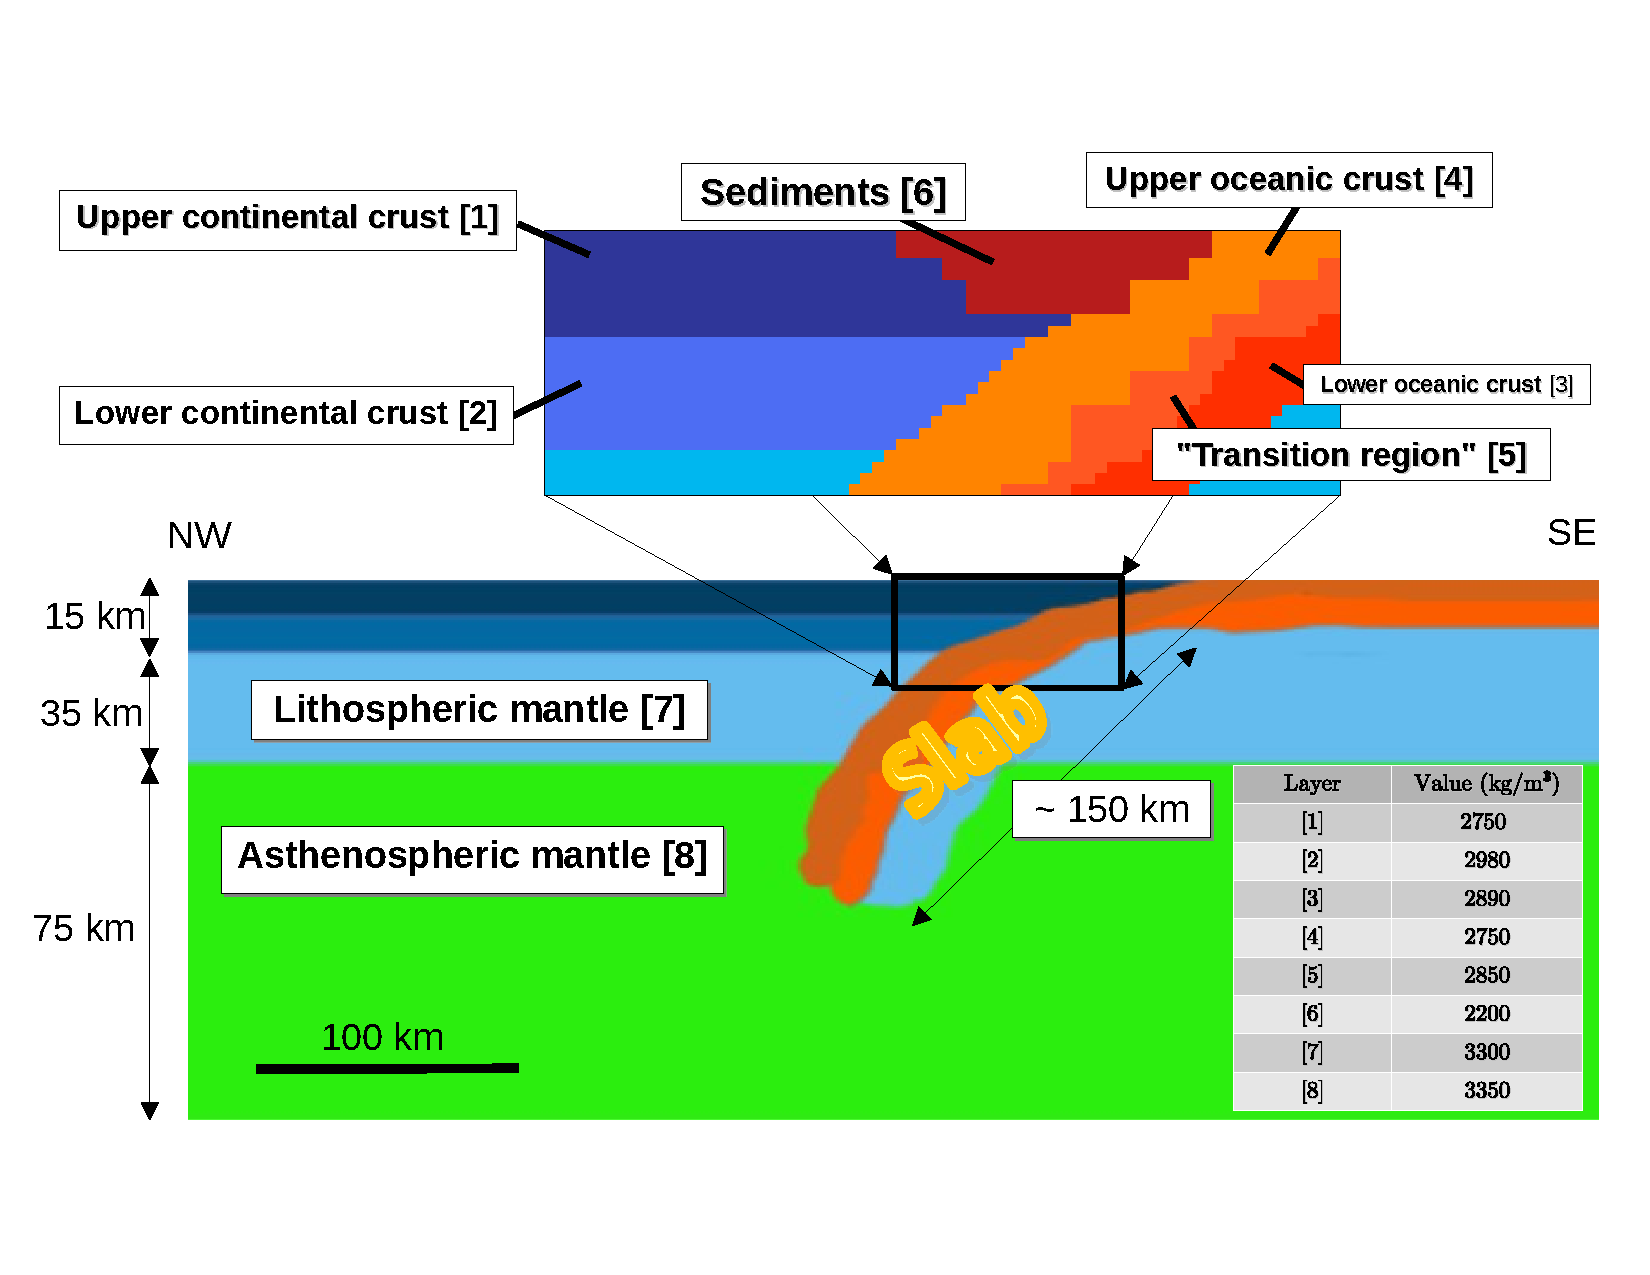
\includegraphics[width=0.65\linewidth]{/figs/slab_model.png}
    \caption{\textbf{Description of the slab model}. A relationship between slab density, slab geometry and subduction rate from theoretical models has been done by studying results of the time-history of the Ionian basin arc. Despite the extensive literature on subduction process, only a handful of studies have examined the role of variable slab buoyancy in the subduction process in the Ionian basin arc geometry \cite{Akimbekova2023}.}
    \label{fig:slabmodel}
\end{figure}
There is of course a first-order discontinuity surface between the crust and the mantle, where the seismic wave velocity rises sharply, namely the Moho surface (transition from crust to mantle). 
\begin{figure}[H]
    \center
    \includegraphics[scale=0.27]{/figs/ak135.pdf}
    \caption{The AK135 model of P velocity ($v_{P}$), S velocity ($v_{S}$) as a function of depth in the Earth \cite{kennet1995}. It has been served the seismological community as a reasonable and reliable reference model for almost 30 years; Source: \url{http://ds.iris.edu/spud/earthmodel/1568955}.}
    \label{fig:ak135}
\end{figure}
Therefore, earthquake sources at different depths in the crust will produce seismic phases with different ray paths at different epicentral distances. The Moho naturally gets deeper when one reaches continental crust, but the followed mesh modeling process did not account for the geometrical distribution of these layers. 
\section{Source characteristics, model and mesh key aspects}
The 1D model consisting of three homogeneous layers is meshed with rectangular elements of a non uniform element size in the global domain. Following the Harvard centroid moment tensor (CMT) catalog solution (Harvard Seismology Group, Cambridge USA), a single point source has been placed in the mesh at various depths, (shown as beach balls on fig. \ref{fig:stfs}) with a quasi-Heaviside "smoothed" step function with an half-duration such that the corresponding moment-rate function is a Gaussian one having a dominant frequency $f_0$ for each kind of mesh. The triangular one is represented to highlight the difference in shape and frequency content. All source-time functions (STFs) must match the duration of their corresponding seismic traces. For instance, a Gaussian STF, which is similar to a triangle with a 2.5 s half-duration, lacks significant energy at periods shorter than 1 s. In contrast, a cosine STF exhibits more energy at higher frequencies. This distinction is important, because the shape of the STF controls the frequency content of the simulated seismogram. If the duration or the shape of the source used in the model do not match reality, spurious energy peaks at specific frequencies may be generated.\\
\begin{table}[H]
    \begin{center}
     \begin{tabular}{|c|c|c|c|c|c|} 
	  \hline ID&EQ (date time) &  $Lat \,(^\circ)$ & $Long \, (^\circ)$  &  $M_w $ & Depth (km) \\ 
	  \hline
 A1&20221012224455.0&38.836&16.653 &4.3  &35   \\
A2&20120704111209.8 & 37.474&16.798 &4.5  &38.4	 \\ 
A3&20250416012608.7& 37.586&16.170 &4.7  &39\\
A4&20140405102446.1& 38.820&17.180 &4.8 &64  \\
A5&20151117071008.8& 38.759&20.451 &6.5 & 10 \\
A6&20181025225451.5&37.533&20.618	 &6.8 & 10 \\
A7&20200321004951.8&39.300&20.620 & 5.7& 7 \\
A8&20220908073624.5&37.973 &20.061& 5.5& 10 \\
A9&20240329071249.1&37.325&21.310& 5.9&  35\\
B1&20200224160217.0&39.360&16.241&4.3& 9.1\\
B2&20241128235415.0&39.210&16.359&4.1&24.1\\
B3&20240529120713.0&39.648&16.986&4.0&24.8\\
B4&20220120091957.0&39.390&16.217&4.3&9.1\\
      \hline
    \end{tabular} 
   \end{center}
   \caption{\textbf{Simulation names, location and relevant information for the seismic sources implemented in each forward simulation}. The last four rows indicate the earthquakes showed to highlight the seismicity of the area.}
   \label{tbl:eqdata}
\end{table}
In the Table \ref{tbl:eqdata} the earthquakes used in all the runs have been indicated, highlighting their most important properties needed to implement them in the SPECFEM code. The earthquakes reported in the event list are in UTC time (Universal Time Coordinated).
In Table \ref{tbl:mtsol} instead, the information about the moment tensor component for each seismic source has been represented. High uncertainty is associated with the inverse solution of the 2012 Ionian earthquake moment tensor components (A2), primarily due to the poor seismograph coverage at that time. This prevent the possibility to obtain precise location and moment tensor analysis of earthquakes that occur in the Ionian Sea far from the coast.
\begin{table}[H]
\centering
     \begin{tabular}{|cccccc|} 
	  \hline Name & Depth (km)  &  $V_{p,max} \, (km/s)$ & $V_{s,min} \, (km/s)$ &     $\rho_{max} \, (\frac{g}{cm^3})$	& $\rho_{min} \, (\frac{g}{cm^3})$	 \\ 
	  \hline
Triple layer  & 80  & 8.00  & 3.37 & 3.30&2.70 \\
ICLARC3D & 80 - 112.5& 8.44  & 2.37 &3.48&2.50	 \\ 
ICLERC3D  &200 - 230 & 8.44  & 2.37 &3.48&2.50 \\
      \hline
    \end{tabular} 
    \caption{\textbf{Triple layer crustal model and 3D model parametrization}. The runs with attenuation shell around the mesh used the same models reported in the last two rows and an homogeneous model inside the shell layer.}
\label{tbl:infosims}
\end{table}
\begin{figure}[H]
\center
    \begin{subfigure}[c]{\textwidth}
        \includegraphics[width=\linewidth]{/figs/stfs_fin.png}
            \caption{}
    \label{fig:stfs}
    \end{subfigure}
            \begin{subfigure}[c]{0.6\textwidth}
        \includegraphics[width=\linewidth]{/figs/finaleSetB.pdf}
        \caption{}
    \label{fig:setB}
    \end{subfigure}
    \caption{(\textbf{a}) Schematic examples of source time function (STF) complexity in time and frequency domain in representative runs with the associated moment tensor focal mechanisms. (\textbf{b}) Closeup view of the enclosed area of the nearest stations to the earthquakes reported in the set B.}
    \end{figure}
\begin{figure}[H]
    \center
    \includegraphics[width=0.85\linewidth]{/figs/mts.pdf}
    \caption{Full moment tensor point source solutions are needed to implement the desired earthquake characteristics in the simulation. In each run, a single earthquake was defined at the epicenter within the corresponding computational grid coordinates.}
    \label{tbl:mtsol}
\end{figure}
In the ICLARC and ICLERC models the material properties defined in the ASCII files, for each single mesh, have been defined with precise spacing criteria: in the horizontal plane a 0.02° by 0.016° grid (respectively longitude and latitude) has been defined while every 2.5 km along the depth a new layer has been defined. After reading the sequential file, a Python interpolation routine was applied in such a way to match the number of nodes defined beforehand, to reach overall stability in the subsequent forward simulations. P and S waves behave differently in the input model. Sharp velocity contrasts between rigid rocks and soft sediments trap seismic energy in specific areas. S waves are more sensitive to this trapping effect: they reflect multiple times within low-velocity layers, increasing amplitude and duration at higher frequencies. P waves show similar but weaker amplification and prolongation effects.
The source wavelet is always centered at time 0.0 s and the simulation start time ($t_0$) is then chosen such that the initial source strength is very close to zero, to avoid high-frequency wave artifacts that would occur if the wave simulation started off with a strong initial source acceleration offset at the source grid points. So, after the mesh has been generated, the minimum resolvable period has been determined verifying that the dominant period, associated either to the external STF or the default smoothed Heaviside one, was greater than the domain's minimum resolvable period. The condition for a good resolution in all simulations has always been $h \le v_{max} / f_{max}$, with $f_{max}= 1 / T_{min} $. It is a necessary condition, but not always sufficient: in practical terms, the minimum resolvable period is the shortest period that the simulation can reliably resolve, given the numerical mesh resolution (element size), the material velocities ($v_S$, $v_P$), the number of grid points per minimum wavelength required for accuracy \cite{komatitsch2005}. 
\begin{figure}[H]
    \centering
        \includegraphics[width=0.55\linewidth]{figs/trpl_ly_mdl.pdf}
		\includegraphics[width=0.35\linewidth]{figs/vrtcl_spacing.pdf}
    \caption{\textbf{Model geometry and mesh simulation setup}. \textbf{Right panel}: 1D velocity model used during the interpolation step for the validation tests. \textbf{Left panel}: Vertical cross-section of the mesh element spacing.}
    \label{fig:1dmodel}
\end{figure}    
The analytical resolvable period, computed based on the chosen mesh, determines the frequency content of the STF chosen to make the convolution as a post-processing step. The numerical Green's functions are indeed valid down to a minimum period determined by the mesh resolution, so frequencies higher than this numerical cutoff may be affected by either numerical dispersion or unstable wave propagation, especially for high-frequency content body waves.
\begin{figure}[H]
    \centering
        \includegraphics[height=6.5cm, width=0.9\linewidth]{figs/vp_trplly+topo.pdf}\\
        \includegraphics[height= 5.6 cm, width=\linewidth]{figs/topo_zoom.jpg}
 \caption{3D perspective view with topography, Moho and interfaces. The topography relief reports DTM levels with accuracy up to 90 m.}
 \label{fig:geom.mesh}
\end{figure}
By plotting the spectrum of the selected source, namely the spectrum of the slip rate functions or the moment rate functions (i.e. derivative of the STF), if the spectral amplitude decayed rapidly enough with increasing frequency, then the STF was implemented in the simulation. Also, if the relative amplitude is small enough at frequencies close to $v_S / h_{min}$ then the source was good enough to be imported in the simulations. If that was not the case, a post-processing operation (low-pass filter) on the synthetics or a mesh refinement (i.e. reducing the smallest element size in order to resolve those high frequencies) was performed.
In simulations A1 - A3, the STF was set to a Gaussian function with a half-duration of 0.6 s. Simulation A4 used a Dirac delta function instead. For simulations A5 - A8, a Gaussian function with a duration of 1.5 s was chosen for the 80 km deep mesh, followed by a cosine function with a half-duration selected based on the magnitude of the chosen event ranging from 1.7 s up to 6.3 s. In some spurious simulations no external STF was selected to convolve with the synthetics, but instead the default smoothed Heaviside step function was convolved with the synthetics (see manual page 42). All figures have been made using SAC \cite{goldstein2005sac} and GMT \cite{gmt}.\\ 
The procedure involved extracting coordinates from the six-column model file, with z-values starting from the surface equivalent to the bathymetry sea level. The mesh files were then generated in CUBIT format, defining depth until the code established a perfectly rectangular area. This area was subsequently read by the code for decomposition and interpolation with the 3D model file in .xyz format.
Particular care was taken to ensure the areas defined in both the model and mesh files matched, and to avoid distortion effects from the interpolation routine, when extruding the mesh area from topography values. The refined mesh at the surface naturally requires more computational time, but this is balanced by coarsening the mesh as depth increases. The topography was therefore clipped to 1.4 km altitude with respect to the sea level surface. This approach was chosen because the highest station elevation in the SeismoCal network is located well below the refinement threshold, making it unnecessary to model higher elevation points that could introduce instabilities and increase computational costs, even though the highest points in the region are in the Pollino range. Serra Dolcedorme, in the Mt. Pollino range, with 2267 m asl is Calabria's highest peak. Nonetheless, no differences were observed when comparing synthetic and real traces in terms of shape and amplitudes, as a result of this clipping. A particularly problematic earthquake (A4) was later simulated using a small mesh defined within the ICLARC model region. The earthquake source location for this seismic event is likely incorrect according to current models proposed for the Calabrian arc subduction region. This event was chosen to test how well the proposed model matches actual seismic recordings.\\
The characteristic parameter of anelastic attenuation is the quality factor Q, defined as 
\begin{eqnarray}
\frac{1}{Q}=-\frac{\Delta E}{2 \pi E}
\end{eqnarray}
where the right-hand side represents the energy variation per unit of total energy dissipated in a cycle by a wave propagating through an anelastic medium. Therefore, strongly attenuating media exhibit very small Q values, while high Q values correspond to weakly attenuating media. Additionally, there is a strong correlation between high-frequency signals and attenuation; however, the frequency dependence of the attenuation factor in solids remains practically constant within the seismic frequency range (i.e. $10^{-3} \, Hz < f < 10^{2} \, Hz$).\\ 
SPECFEM models attenuation using a constant quality factor Q, approximated through a series of Zener standard linear solids (SLS) rather than direct implementation. This approximation is valid only within a specific frequency band centered on the reference frequency, which corresponds to the maximum frequency resolvable by the computational grid. Therefore, the model's quality factors remain constant within this frequency range, following the SLS approximation baseline around the reference frequency.\\
No attenuation is considered in the first simulations, i.e. the attenuation parameters $Q_{\kappa}$ and $Q_{\mu}$ are set internally by the interpolation routine to 9999, to simulate purely elastic wave propagation, without any attenuation effects which will introduce a factor $1.5$ into the computation costs \cite{martin2008}. A 33 km thick shell layer was subsequently defined in the horizontal directions (UTM-E, UTM-N) with $Q_P$ and $Q_S$ values of 10 and 20 respectively to mitigate unwanted reflected phases. The bottom 30 km layer of the mesh was also defined as anelastic (see Figure \ref{fig:guscio} and \ref{fig:iclarc_scheme}). The equivalence between the two sets of attenuation factors is reported below, the difference nevertheless is of the order of unity
\begin{align}
Q_{P}^{-1} &= \left(1-\frac{v_{S}^{2}}{v_{P}^{2}}\right)\,Q_{\kappa}^{-1}
              + \frac{v_{S}^{2}}{v_{P}^{2}}\,Q_{\mu}^{-1},\\
Q_{S}^{-1} &= Q_{\mu}^{-1}.
\end{align}
\begin{figure}[H]
\centering
        \includegraphics[height=5.5 cm, width=0.9\linewidth]{figs/shell_mesh.jpg}
\caption[]{Both models later incorporate an attenuation shell that serves as an absorbing layer where the wave field is damped by propagation through a strongly attenuating medium (characterized by low $Q_P$ and $Q_S$ values). This approach must be calibrated with the recording time defined for synthetic acquisition: longer recording times require stronger attenuation and greater shell thickness.}
\label{fig:guscio}
\end{figure}
\section{Code validation by a test of homogeneous triple layer}\label{sez:codevalid}
An horizontally homogeneous three-layer structure has been interpolated to the selected mesh since no accurate results could be extracted if a portion of the proposed 3D model were to be interpolated to the selected smaller grid portion. Nevertheless, to discriminate the known effects the topography can introduce in the synthetics phase characteristics, the mesh has been defined having and not having it: in this way the synthetics in the two cases have been compared with the real data (respectively FLAT and TOPO in Figure \ref{fig:mesh_czlido}). The selected mesh for the A1 seismic source contains 530,000 elements, with 100 grid points in each horizontal direction and 53 points along the z-direction. The average spacing is $\Delta x$=790 m, $\Delta y$=734 m,  $\Delta z$=943 m. The mesh coordinates range from 16.10°E to 16.53°E longitude and from 39.25°N to 39.46°N latitude. To realistically capture the regional geometry, a 3D model constructed from bathymetry and topography data is required to account for topographic and even oceanic effects on wave propagation. The Figure \ref{fig:section_czlido_iclarc} shows a portion of grid points assembled for the synthetic waveforms computations with values of density-velocity parameters for cuts along the latitude (Y) and longitude (X). Once the synthetic signals are obtained, the comparison procedure requires an appropriate filtering of real data to reduce their frequency content to the same of the synthetic traces. Waveforms are being shown in units of displacement of the ground in each direction, filtered with the following time windows (10 - 30 s periods). The real data is shown with black line while the synthetics in red.
\begin{figure}[H]
    \centering
 \includegraphics[height=6 cm,width=0.8\linewidth]{figs/mesh_czlido.jpg}         \\ \includegraphics[height=4.5 cm, width=0.7\linewidth]{figs/mesh_flat.pdf}
    \caption{Comparison between meshes with and without topography (FLAT and TOPO cases). The CZLIDO mesh shows the triple-layer model following the interpolation routine.}
    \label{fig:mesh_czlido}
\end{figure}
 The 3D model is characterized by thin oceanic crust throughout most of the Ionian basin, with the Moho discontinuity deepening as it approaches both the Calabrian and Hellenic arcs. The two subducting slabs (Calabrian and Hellenic) are modeled by varying $v_P$, $v_S$, and density using reasonable parameter values. Since subducting slabs sink into the mantle, their density must exceed mantle density at equivalent depths. Furthermore, given the very low thermal conductivity of rocks, subducting slabs remain colder than the surrounding mantle; therefore, seismic wave velocities are slightly higher than those in the ambient mantle at the same depth. The 3D model is expected to produce superior results compared to the three-layer model, particularly for regional earthquakes such as those located in the Hellenic arc. The main challenge when modeling Earth's crust properties with a certain degree of accuracy, is that crustal structure cannot be easily represented by applying perturbations (such as Gaussian noise) to smooth "background" models. This limitation means that the model does not adequately consider vertical cross-sections of compressional wave-speed perturbations. Moreover, no real knowledge can be safely stated about the material properties in the subsurface region.
\begin{figure}[H]
    \centering
        \includegraphics[width=1.1\linewidth]{figs/sezioni.czlido.pdf}\\
         \includegraphics[width=1.1\linewidth]{figs/sezioni.iclarc.pdf}
    \caption{\textbf{Simulation model setup}. The top row shows the model used in validation tests, while the bottom panel displays a latitude cross-section at 38.5° N of the ICLARC model. Both rows present: (a) compressional wave velocity, (b) shear wave velocity, and (c) density.}
    \label{fig:section_czlido_iclarc}
\end{figure}
In the Figure \ref{fig:realivssynczlido} the ground motions of the best stations with good SNR have been shown, sorted by distance from the earthquake hypocenter.
\begin{figure}[H]
    \center
    \includegraphics[width=0.9\linewidth]{/figs/confronti/3strat-bccatlidovs20221012_topogra.pdf}
    \caption{Comparison of the Z component observed ground displacement waveforms and the synthetic velocity waveforms filtered in 0.1 - 0.3 Hz band, located at roughly 5 km (SW direction) of the A1 earthquake hypocenter. The units of displacement are micrometers (Up and down).}
    \label{fig:realivssynczlido}
\end{figure}
\begin{figure}[H]
    \center
    \includegraphics[width=0.9\linewidth]{/figs/confronti/notoposilavsreali.pdf}
    \caption{Comparison of the observed and the synthetic ground displacement waveforms in 0.1 - 0.3 Hz band, for the A1 earthquake in the case of the FLAT mesh. The units of displacement are micrometers.}
    \label{fig:synnotopo}
\end{figure}
Comparison between synthetic seismograms with and without topographic effects reveals minimal differences (Figure \ref{fig:synnotopo}); it's always convenient though to implement the topography in the mesh modeling phase, since high frequencies can safely be resolved with the grids designed with the non honoring mesh approach. However, when synthetic seismograms incorporating topography are compared with observed recordings, notable distinctions emerge (see Figure \ref{fig:realivssynczlido}). S wave arrivals and waveform characteristics show good agreement for recordings from nearby stations. This correspondence deteriorates with increasing source distance, where synthetic-observed agreement becomes less evident.
\section{Simulation in a fully parametrized subduction zone with an attenuating shell layer}\label{sez:subductzone}
In the next step numerical seismograms from more wavefield simulations were analyzed, by varying model parameters and examining the resulting waveform changes. A quantitative comparison of synthetic ground motions with available recorded data obtained from stations throughout the Calabria's continental crust is provided. The investigation continued with computational domains discretized up to 80 km depth level, which were subsequently extended to encompass domains of 200 km depth. The analysis employed a three-dimensional model specifically developed for the study region, both for the ICLARC and ICLERC model, which was then replaced by a hypothetical three-layer crustal model, with underlying layers derived from the 1D radial structure of the Earth defined in the AK135 reference model (\cite{kennet1995}, see Figure \ref{fig:ak135}), since the region of investigation is contained in the first crustal layers. 
The mesh properties correspond to the details described in the previous sections: only the number of grid points was slightly modified along each direction, always making sure the selected choice satisfied to the fullest the stability criteria. 

\begin{figure}[H]
    \centering
        \includegraphics[width=\linewidth]{figs/figure_greece2.png}
    \caption{\textbf{Description of the geometry area of the 3D ICLARC model region}. The section corresponds to the 39° N latitude. The region highlighted in blue shows instead the extended area, where the Greece earthquakes have been simulated.}
    \label{fig:iclarc_scheme}
\end{figure}
Compared to the real data, the numerical seismograms (ICLARC and ICLERC models) in the A3 source case are more similar (Figure \ref{fig:realivs3dIONIO25e12}) than with the A2 case, as this is the case when the waves propagate in a medium which tries to mimic the real Earth's structure rather than an homogeneous structure.
Quantitatively, one can see in Figure \ref{fig:syn3dvs3strIONIO25e12} that the first numerical waveforms of the ICLARC models are overall more similar to the real traces compared to the homogeneous model synthetics.
\begin{figure}[H]
    \center
    \includegraphics[height=5.4cm, width=0.8\linewidth]{/figs/iclarc_vp.png}\\
    \caption[]{Interpolated 80 km deep mesh with the ICLARC 3D model. The material property shown is the compressional P wave velocity.}
    \label{fig:mesh_iclarc}
\end{figure}
The SEM data, generated with a very high sampling frequency, is later decimated to a time step of 0.01 s to have the same sample rate of the real data. After detrending and subtracting the mean of each ground motion, since the SEM synthetics are accurate for a specific frequency range, based on $T_{res}$, the whole real and synthetic traces are filtered over a specific frequency range. The synthetics have been convolved with a Gaussian STF of 1.5 s half duration. The duration of seismograms recorded at the Earth's surface depends on both the extent of seismic rupture (and consequently fault size) and the heterogeneity of the medium through which waves propagate from source to receiver. More specifically, seismic event duration is controlled by the geometry and final extent of the rupture front, rupture velocity, and the relative position between receiver and source. For the ICLARC mesh, 100 s long three-component seismograms at all 85 stations have been simulated while the bigger ICLERC one extended the duration to 240 s.
\begin{figure}[H]
\center
\includegraphics[height=7.25cm, width=\linewidth]{/figs/confronti/3d2025vs3st2025.pdf}\\
\includegraphics[height=7.5cm,width=\linewidth]{/figs/confronti/3d2012vs3st2012.Z.pdf}
\caption[]{Comparison of synthetic ground displacement waveforms for various input models in the 0.07 - 0.3 Hz frequency band for the A3 and A2 earthquake respectively. Both computational meshes extend to 80 km depth level, with displacement units in micrometers.}
    \label{fig:syn3dvs3strIONIO25e12}
\end{figure}
At some stations (Figure \ref{fig:syn3dvs3strIONIO25e12} CEL, TIP), the homogeneous model may still perform adequately, suggesting that fine layering does not strongly influence wave propagation in those particular source receiver paths. The peak vibration values at MPAZ stations are similar and range in 22 - 11 $\mu$m for horizontal components and from 10 to 15 $\mu$m  for vertical components (at epicentral distances of 124 km).
Figure \ref{fig:realivs3dIONIO2025} confirms that 3D modeling is essential for capturing waveform complexities that are strongly related to lateral heterogeneities, such as sedimentary basins, as expected. These structural features primarily affect the horizontal components, where the improved fit from 3D modeling is particularly evident. Only minor variations occur in the initial seconds of the traces when comparing different structural models. This result is expected because this portion of the seismograms consists of direct waves. \\
\begin{figure}[H]
    \center
    \includegraphics[height=7cm, width=\linewidth]{/figs/confronti/realivs3d2025.pdf}\\
     \includegraphics[height=7cm, width=\linewidth]{/figs/confronti/realivs3d2012.Z.pdf}
    \caption[]{Comparison of real ground motion and synthetic waveforms for ICLARC model in the 0.07 - 0.3 Hz frequency band for the A3 and A2 earthquake respectively, both for 80 km deep computational meshes, with displacement units in micrometers.}
    \label{fig:realivs3dIONIO25e12}
\end{figure}
Seismic wave identification becomes challenging due to complex wave interactions. On horizontal components, SH phases show unclear or reversed polarities, while vertical components contain mixed energy that obscures direct P wave arrivals. This complexity arises because SV phases appear on all components depending on source geometry, making S wave identification difficult. The problem worsens when the velocity model contains discontinuities that cause wave conversions between P and S phases. These complications create unidentified reflected phases that interfere with accurate frequency band selection and reliability of misfit calculations between synthetic and observed data.\\
\begin{figure}[H]
    \center
    \includegraphics[height=7cm, width=\linewidth]{/figs/confronti/3d2012vs3st2012.N.pdf}\\
    \caption[]{Comparison of synthetic waveforms for ICLARC (\textbf{left}) and triple layer model (\textbf{right}) respectively in the 0.07 - 0.3 Hz frequency band for the A2 earthquake, for 80 km deep computational meshes,.The displacement units are micrometers.}
    \label{fig:syn3dvs3stIONIO2012}
\end{figure}
%3dvs3stguscio2014
\begin{figure}[H]
    \center
     \includegraphics[height=7.0cm, width=\linewidth]{/figs/confronti/3dvs3st2014200kmgusci.E.pdf}\\
    \caption[]{Comparison of synthetic waveforms for ICLARC model (\textbf{left}) and triple layer model (\textbf{right}) both with the attenuation shell layer in the 0.07 - 0.3 Hz frequency band for the A4 earthquake respectively, with 230 km deep computational meshes,.The displacement units are micrometers.}
    \label{fig:realivs3dIONIO2025}
\end{figure}
An interesting case is represented by station CEL and JOPP (Figure \ref{fig:syn3dvs3stIONIO2012}), where it is observed that model ICLARC causes strong reflected phases on horizontal components between about 45 s and 60 s. This suggests that the wave speeds reflected along the boundaries are not well represented in the 3D model whereas the role of small-scale layering might generate an amplitude misfit. The 3D model often reduces mismatch in amplitude envelopes, whereas the homogeneous model systematically underestimates or overestimates energy in the synthetics. However these phases in the synthetics may also be simply due to the reflecting boundaries of the computational mesh. However, examining the 40 - 70 s time window closely reveals that the attenuating shell significantly reduces reflected phases at other stations (LADO, PLAC, CUP2).
To a first approximation, Earth can be regarded as spherically symmetric on a global scale or as flat and horizontally layered on a local scale. The theoretical arrival times computed using EQLOC, based on a stratified homogeneous model for the Calabrian region, show good agreement with the 3D model results, as it is shown in Section \ref{sez:misfit}.
In Figure \ref{fig:3dgusciovs3d2014} the A4 earthquake has been simulated varying the input model exchanging the 3D model with the triple homogeneous layer to see the difference in the waveforms and to later compare the traces with the real data. The synthetics have been convolved with a cosine taper function with an half duration of 2 seconds.
\begin{figure}[H]
    \center
    \includegraphics[height=6.0cm, width=\linewidth]{/figs/confronti/3dgusciovs3d20142014200km.N.pdf}\\
     \includegraphics[height=7.0cm, width=\linewidth]{/figs/confronti/3dgusciovs3d2014200km.Z.pdf}
    \caption[]{Comparison of synthetic waveforms for ICLARC model with the shell layer (\textbf{right}) and triple layer model (\textbf{left}) without the shell layer in the 0.07 - 0.3 Hz frequency band for the A9 earthquake respectively, both for 230 km deep computational meshes. }
    \label{fig:3dgusciovs3d2014}
\end{figure}
The signals in Figure \ref{fig:3dgusciovs3d2014} are not displayed in 1:1 correspondence but are arranged to demonstrate results and improvements in reducing shell reflections. The simulation results clearly demonstrate that model changes significantly impact synthetic signals. Additionally, seismic source positioning within different material properties and interfaces substantially affects the accuracy of synthetic-to-observed data comparisons. Indeed great care must be paid when one places the seismic point source between two interfaces which, in some cases, created unwanted numerical errors in the synthetics.
\begin{figure}[H]
\centering
        \caption{\textbf{Shell attenuation layer implemented both for the regional models}. (\textbf{Top}) ICLERC mesh closeup view of the stations throughout the Calabrian region. No topography has been defined in the mesh modeling process along the Hellenic region. (\textbf{Bottom}) ICLERC area with the attenuation shell.}
        \includegraphics[height=9.4 cm, width=0.75\linewidth]{figs/mesh_gree.jpg}\\
        \includegraphics[height =9 cm, width=0.85\linewidth]{figs/figure_greece.pdf}   
\end{figure}
In the ICLERC mesh the same approach was followed as before but the area was much larger extending to two different UTM zones. For this reason, a Lambert projection has been applied to accurately represent the study area. With distances up to 500 km that characterize this model the Earth's curvature should be taken into account, but due to time constraints, the Globe version of the code has not been used in this work. In this region, the 3D model is specified into 267 elements along each direction with element size at the surface as 1.69 km times 1.59 km. As depth increases, the computational grid is characterized by two layers, where the lower section exhibits a significant node reduction, such that the mesh element size reduces from the latter value to 2.69 km. 
\begin{figure}[H]
    \center
    \includegraphics[height=8cm, width=0.97\linewidth]{/figs/confronti/macro.3D3strati.cutr.jpg}\\
     \includegraphics[height=7.5cm, width=0.97\linewidth]{/figs/confronti/macro.sismZsintreali2.png}
    \caption[]{\textbf{Top panel}: Comparison of synthetic waveforms for ICLERC model and triple layer model in the 0.1 - 0.3 Hz frequency band closest to the A9 earthquake, both for 80 km deep computational meshes, with displacement units in micrometers. \textbf{Bottom panels}: Comparison of real and synthetic Z component waveforms for the same A9 earthquake and frequency band. The stations name matches with the traces order.}
    \label{fig:reali3DGRE2024vari}
\end{figure}
The waveforms of long-period surface waves from Greek seismic sources are accurately resolved when compared with observed data. It must be taken into consideration that many uncertainties are present in the estimated focal mechanism and depth of the source, which might modify slightly the S wave radiation pattern. The analysis of the differences between the seismograms produced by this type of simulation and those actually measured offer crucial information to determine the characteristics of the basin arc proposed model and its response to hypothetical seismic events.
\begin{figure}[H]
    \center
    \includegraphics[height=8.75cm, width=\linewidth]{/figs/confronti/realivs3d201880km.E.pdf}\\
     \includegraphics[height=8.75cm, width=\linewidth]{/figs/confronti/realivs3d201880km.Z.pdf}
    \caption[]{Comparison of real ground motion and synthetic waveforms for ICLERC model in the 0.07 - 0.3 Hz frequency band for the A6 earthquake respectively, both for 80 km deep computational meshes, with displacement units in micrometers.}
    \label{fig:realivs3dGRECIA201880km}
\end{figure}
On the other hand Love waves are expected not to be important in the 1 - 10 Hz frequency range for local small earthquakes, as it was never the case to reach such a period time window.  It was also noticed that the computed Rayleigh waveforms have overestimated amplitudes when compared to real surface waveforms after 80 s, as it's shown for the A6 earthquake (Figure \ref{fig:realivs3dGRECIA201880km}).\\
\begin{figure}[H]
    \center
    \includegraphics[height=7.55cm, width=\linewidth]{/figs/confronti/synt.3d2022vs3st.Z.pdf}\\
     \includegraphics[height=7.55cm, width=\linewidth]{/figs/confronti/synt.3d2022vs3st.E.pdf}
    \caption[]{Comparison of synthetic waveforms for ICLERC model and triple layer model in the 0.07 - 0.3 Hz frequency band for the A8 earthquake, both for 80 km deep computational meshes.}
    \label{fig:3dvs3st2022GRE80km}
\end{figure}
When more detail was required for the surface waves, especially with the very distant Greece earthquakes, a broader frequency range was selected to ensure a good fit with the Love and Rayleigh arrivals. In Figure \ref{fig:sections_iclerc} some sections of the 3D tomographic model used in this simulation are represented, the colors represent the different speeds of the seismic waves, from red (8 km/s) in areas with higher speeds up to dark blue (3.35 km/s) in the slowest areas. 
On the contrary, in the A8 case (Figure \ref{fig:3dvs3st2022GRE80km}), the amplitudes of surface waves are similar to the amplitudes of the experimental data, which is very encouraging. As it can be seen in the recorded data,  the S wave dominates but the P wave and surface waves are also clearly visible.
\begin{figure}[H]
    \centering
        \includegraphics[width=1.1\linewidth]{figs/sezioni.iclerc.pdf}\\
         \includegraphics[width=1.1\linewidth]{figs/sezioni.iclerc3st200km.pdf}
    \caption[]{\textbf{Simulation model setup}. The top row shows an ICLERC model latitude cross-section, while the bottom panel display the extended triple layer model up to 230 km depth level. Both rows present: (a) compressional wave velocity, (b) shear wave velocity, and (c) density.}
    \label{fig:sections_iclerc}
\end{figure}
\begin{figure}[H]
    \centering
        \includegraphics[width=1.1\linewidth]{figs/sezioni.iclarcG.pdf}\\
         \includegraphics[width=1.1\linewidth]{figs/sezioni.iclercG.pdf}
    \caption{\textbf{Simulation model setup}. The top row shows the ICLARC model latitude cross-section at 38.5° N used with the attenuation shell layer, while the bottom panel displays the ICLERC with the shell layer. Both rows present: (a) compressional wave velocity, (b) shear wave velocity, and (c) density.}
\end{figure}
It can be observed from Figure \ref{fig:realivs3dGRE24e18} that the peak amplitude of the synthetics can be captured and they match closely with the recorded ground motion in the selected frequency range capturing well enough the P wave polarity. Far-field stations can capture frequencies up to 0.2 Hz and near-field can capture frequencies up to 0.35 Hz. This frequency window range, used when filtering most of the data, was selected since the typical range for regional events is between 0.05 Hz and 2.0 Hz; one common choice is to set the low-cut frequency to around 0.1 Hz to remove long-period noise while preserving the main SNR. A reasonable range for high-cut frequency with an half duration of 0.6 s is 1.0 Hz up to 2.0 Hz, which can effectively filter out high frequency noise. It is also advisable to select a consistent time window and maintain the same interval throughout the analysis to avoid introducing bias and eliminate spurious results that may arise from subjective parameter choices.
\begin{figure}[H]
    \center
    \includegraphics[height=7.5cm, width=\linewidth]{/figs/confronti/realvssynt2024200km.N.pdf}\\
     \includegraphics[height=7.5cm, width=\linewidth]{/figs/confronti/realivssynt2018200km.N.pdf}
    \caption[]{Comparison of real and synthetic waveforms for ICLERC model in the 0.07 - 0.3 Hz frequency band for the A9 earthquake and A6 respectively, both for 230 km deep computational meshes.}
    \label{fig:realivs3dGRE24e18}
\end{figure}
All these results show the crucial importance of the data sensitivity to the source modeling and particularly to the source location at depth. Since these P phases are more pronounced, the SV wave phases in the vertical plane are less and less visible even if they are still existing. In any case, these preliminary observations and results obtained seem to indicate that the simulated signals are recorded with a good SNR for small earthquakes ($M_{w}< 5.0$) at regional distances and even with far more accuracy for far earthquakes with $M_{w}> 5.5$. 
In view of the above discussions, the role of the three dimensional heterogeneous velocity structure in the moment tensor point source during large earthquakes should be studied in more detail by accumulating knowledge from such large crustal earthquakes. A higher resolution velocity model in the target area would help investigate the spatial relationship between possible future strong earthquakes and the heterogeneous crustal structure. It's also a well known fact in earthquake seismology, that the hardest seismic parameter to constrain is the rock density, because most seismic observables are generally insensitive to this parameter, even though in exploration seismology the reflected waves employed are sensitive to impedance constraints (i.e. product of density and wave speed). Obtaining high-quality measurements for data analysis is still challenging with current HPC (High Performance Computing) centers, as the data volume required to improve the starting model frequently reaches terabytes of earthquake recordings, creating significant I/O handling issues.
Love waves, a type of surface wave, are clearly observed on the East component because they consist of horizontally polarized S-waves trapped within low-velocity layers. When source locations are very deep, surface wave amplitudes are naturally much smaller. Therefore, the depth information for the Greek earthquakes (A5 - A9) requires careful consideration. The similar amplitudes are likely due to a significant surface wave contribution, which is consistent with the shallow source depths of the earthquakes (10 - 29 km). However, these depths can have uncertainty of several km due to the poor seismic station coverage in the Hellenic arc.\\
Unfortunately the unwanted reflected phases coming from the mesh boundaries are clearly visible, most likely also in the 80 s mark (see Figure \ref{fig:realivs3dGRE24e18}) and on where the onset of the surface waves is disturbed by these unnecessary phases. 
No definitive conclusion can be drawn, whether this procedure effectively reduces reflected phases in the seismograms or not. Additional simulations are required to determine whether this approach yields meaningful improvements or provides no substantial benefit.\\
Overall, both proposed 3D models successfully reproduce (and occasionally overestimate) many features observed in seismograms across all components; however, further improvements could be achieved with relatively modest effort.
\section{Further synthetics preliminary results}\label{sez:discussion}
Snapshots of seismic wave propagation derived from the SEM simulation for the A3 earthquake, that display the way in which the regional wavefield spreads from a shallow source in the Calabrian arc, are shown in Figure \ref{fig:video}. In order to compensate for the geometrical attenuation of the body waves and to improve the visibility of the seismic phases in the later time frames, a zero half duration was defined in the moment tensor point source file to accurately represent the seismic wavefield as it propagates in the grid domain. What actually defines the limit band of frequencies, which can be accurately depicted in the video simulations, are roughly defined by
\begin{eqnarray}
f_{v} \simeq \left[0, \text{min}\left(\frac{1}{2\Delta t}, \frac{ v_{s,min} n_{ppw}}{(N+1) h_{min}}\right) \right],
\end{eqnarray}
where $n_{ppw}$ is the required number of GLL points per wavelength for accurate resolution, $\Delta t$ is the simulations time step, $h_{min}$ is the minimum element size in the mesh, $v_{S,min}$ is the minimum shear-wave velocity in model and $N+1$ is the number of GLL points along one element edge. The lower frequency bound defines the Nyquist frequency. In other words, by setting a null half duration, no characteristic frequency is imposed by the source. Each frame of the video has been acquired every 200 time steps of the real 3D wavefield simulation. Later on, the seismograms and the evolution of the ground velocity values on the whole mesh free surface are saved and displayed through Paraview. 
\begin{figure}[H]
    \center
    \includegraphics[scale=0.4, height=6cm]{/figs/snapshot3d.png}
    \includegraphics[scale=0.4, height=6 cm]{/figs/snapshot3d2.png}
    \caption{\textbf{3D wavefield animation}. Snapshots at different time steps of the vertical-component velocity wavefield of the 2025 Ionian earthquake propagating along the surface. Red denotes negative values and blue positive values. The view is from the $+\hat{z}$ direction. }
    \label{fig:video}
\end{figure}
To reduce calculation times and given the limited current knowledge of subsoil details, the simulation in this animation is showing relatively "low-frequency" waves, down to 0.125 Hz, since an external cosine function of four seconds half duration has been employed. This means that the wave front "interacts” with objects of ten km in terms of size, well above the threshold introduced with the STF selected in the moment tensor point source solution.\\
The frame index is directly related to the actual time in the simulated 3D wavefield, since each time index reported is given by the time step at the frame number starting from 1 multiplied by the time step chosen to integrate the wave equation. Each second of the animation corresponds to one second of real time. A coast relief and 16 representative stations with a good SNR quality have been reported in the video. The elapsed time is intended in the sense that it's the time passed since the earthquake point source has been placed in the domain (that is the time since the earthquake origin time). 
Color intensity corresponds to the vertical velocity, with more intense colors indicating faster motion. The anisotropic feature of the seismic source is clearly recognized in the amplitude depending on the azimuth. The color gradation represents vertical velocity values (m/s), where more intense blue (or red) indicates faster upward (or downward) ground motion. The speed and amplitude of seismic waves depend on seismic source characteristics, subsurface material properties, and topographic features. Consequently, wave propagation is non-uniform in space, causing locations equidistant from the epicenter to experience significantly different ground displacement.\\
The animation demonstrates heterogeneous ground velocity distribution, meaning that points equidistant from the epicenter experience different stress patterns. This variation results from local conditions, including topography, soil type, and site effects, that significantly influence seismic wave propagation.
By comparing the simulated and real seismic data some important results can be assessed: both the polarity and amplitude of the first P wave is practically identical, even though some unknown phases seem to appear in the vicinity of the S wave first arrival, which are likely due to the Stacey absorbing boundary conditions.

\begin{figure}[H]
    \center
   % \includegraphics[width=\linewidth]{/figs/confronti/diff.fasePnogusciosiguscio.2025.png}\\
    \includegraphics[width=0.9\linewidth]{/figs/confronti/closupfasiP.3d2025.pdf}
    \caption{Closeup comparison of P wave arrivals along the Z component waveforms filtered in the  $f_1$ band for the A3 earthquake, with displacement units in micrometers. The amplitudes have been clipped to 10 $\mu$m to better illustrate their similarities. }
    \label{fig:difffasiP}
\end{figure} 
The waveforms in Figure \ref{fig:difffasiP} match the P wave polarity but the physical properties of the propagation medium can be better refined to match the observed seismic data.
More care must be given when trying to define the present phases in the synthetic recordings. From the closeup shown above, the anomalous phases could be an artifact generated at the interfaces or it could be the model inconsistency with the actual materials arranged in the modeling. Station GMB1 (Figure \ref{fig:difffasiP}) may be located in a sedimentary basin that naturally traps seismic energy. Increasing the magnitude and spatial variability of attenuation quality factors could improve synthetic-observed data agreement, warranting further systematic evaluation. Future work should address the treatment of sharp Q contrasts, which currently do not generate expected reverberated phases. A more realistic approach would implement smoothly varying attenuation gradients rather than abrupt changes, better matching wave propagation physics in heterogeneous media.
The ICLARC model may not correctly represent the properties (thickness, velocity) of the surface layers, and therefore accentuate this resonance. If the ICLARC model does not include or underestimates the known effects of attenuation (the Q parameter), the energy propagates with minimal loss. In this case, waves propagating along specific paths toward specific stations with known site effects presence, may not dissipate sufficiently, resulting in an overestimation of the amplitude at certain frequencies. This discrepancy could be due to the issues with the mesh discretization or how the code handles the convolution with the external STF, which might introduce frequency spurious artifacts in the synthetics. 
The ICLARC model is based on a grid, which can lead to errors in its discretization. If the grid spacing is too large compared to the wavelength of the frequencies between 14 and 33 seconds used in the filter, numerical errors may arise, leading to artificial amplification. To verify the quality of synthetic results, spectra were computed using SAC.\\
Figure \ref{fig:spettri} shows several key observations: the synthetic spectra exhibit much greater similarity to each other compared to the observed data spectra, which show considerably more variability. This discrepancy highlights one of the primary reasons for the evident differences between synthetic and observed data pairs: the heterogeneities known to exist in the study region have not been accurately captured in the input model used to generate the synthetics.
\begin{figure}[H]
        \begin{subfigure}[c]{0.50\textwidth}
        \includegraphics[height= 4 cm, width=\linewidth]{figs/confronti/spettri.N.2024200kmimp.png}
        \caption{}
    \end{subfigure}
\begin{subfigure}[c]{0.50\textwidth}
             \includegraphics[height= 4 cm, width=\linewidth]{figs/confronti/spettri.N.2024200km3stimp.png}
             \caption{}
\end{subfigure}
        \caption{(\textbf{a}) Normalized Fourier amplitude spectrum for the North component ICLERC synthetic waveforms and the real traces for the A9 earthquake, in the case of 200 km deep computational mesh. (\textbf{b}) Normalized Fourier amplitude spectra for the North component triple layer model. Both sets of signals have not been filtered before computing the spectra and a smoothing and decimation operation has been applied before plotting.}
\label{fig:spettri}
\end{figure}
Additionally, the spectra are strongly dependent on the STF used for convolution, as it can be seen by comparing the STF spectra with the corresponding synthetic spectra. Limited additional information can be extracted from synthetic spectra alone, since the most valuable insights emerge from direct comparison with observed data.\\
No real difference can be gathered by looking at artificial frequency content obtained from known parameters given by the user when one sets up the forward problem. 
%%%%%%%%%%%%%%%%%MISFIT%%%%%%%%%%%%%%%%%%%%%%%%%%%%%
\section{Waveform misfit and model optimization}\label{sez:misfit}
The next step is the improvement of the model, in terms of a chosen parameter (density, velocity, attenuation parameters etc..), based on the data gathered in the forward simulations. One may choose model parameters that describe 3-D elastic structure (i.e. elastic tensor \textbf{C}, density), 3-D attenuation, topography of interfaces (such as Moho honoring and basement surfaces), and earthquake sources (i.e. moment tensor $\mathbf{M}_{ij}$, hypocenter, origin time). The choice of a misfit function for example, waveform, travel time, or amplitude differences will affect the construction of "adjoint sources" which plays a role in the consequent phase along a FWI problem, the so called "adjoint problem".  Selecting appropriate misfit criteria is key to achieving a generally accurate "final" model: this choice is highly dependent on the data quality and frequency ranges of investigation. Naturally it will never be reached a perfectly matched model which can accurately represent the phase arrivals properties registered in real seismograms.\\
L2 norm misfits for the ICLERC and ICLARC models were calculated as the ratio of recorded to simulated ground motion, enabling station-by-station and component-by-component comparisons. Different time windows of [20, 30, 40, 50] s, centered on P and S wave arrivals, were defined to accurately assess the quality of results obtained for the A9 event, which exhibits the best SNR among all simulated earthquakes. By its core, the misfit function sums the least squares difference between observed and synthetic traces for a chosen duration of time and frequency band. 
Later a 30 s  / 35 s  window (P and S wave respectively) were selected for both theoretical time arrivals for representative events which can highlight where the model under performs in terms of accuracy with the underlying Earth's structure. Two earthquakes, one located to the south (A3) and one located to east (A6) are used to compare the normalized cross-correlation to probe different ranges of accuracy defined in the areas with most uncertainty.\\
Firstly the information about the earthquake source coordinates has been assigned for each simulation to all seismic signals. Later on the components between the same same stations of both synthetic and real data have been paired in order to compute the highly non linear L2 norm ($\chi (m)$) and normalized cross correlation ($\mathcal{NCC}(\tau)$) per component per station. Namely
\begin{eqnarray}
\chi (m) \mathop{=} \frac{1}{2} \sum_{i=1}^{N_{r}} \frac{\sqrt{ \int_{W} [d_{i}(t)-s_{i}(t)]^2 dt} }{\sqrt{\int_{W}  d_{i}^2(t) dt} + \sqrt{\int_{W}  s_{i}^2(t) dt}},
\end{eqnarray}
where m stands for the input model used in the forward problem and $N_r$ is the number of receivers for the SEM data. The normalized crosscorrelation has been implemented as the following metric
\begin{eqnarray}
\mathcal{NCC}(\tau) = \sum_{i=1}^{N_{r}} \frac{ \int_{W} [ d_{i}(t) \, s_{i}(t+\tau)] dt }{\sqrt{ \mathop{\int_{W}}  d_{i}^2(t) dt \cdot \int_{W}  s_{i}^2(t) dt }}.
\end{eqnarray}
The removal of the mean, detrending and tapering with Hanning window have been applied, as it is usually the case with the comparison between the two sets of data. No rotation has been applied to the seismic traces before selecting the time window and computing the misfit metric. When considering the instrument and band codes applied to both synthetic and observed data, particular care was taken to distinguish between data quality levels. 
Waveform difference misfit values can be dominated by large amplitude variations, which can mask important phase information. Since amplitude depends on multiple factors (source properties, local structure at source and receiver sites) while phase directly reflects seismic wave velocity, these parameters should be analyzed separately. However, phase-based analysis requires high-quality, low-noise data and similar waveform shapes to avoid phase unwrapping discontinuities that compromise the comparison. Most of the results were therefore analyzed in a low and narrow frequency range between 0.07 - 0.2 Hz and 0.02 - 0.1 Hz for P and S wave respectively. 
\begin{table}[H]
\centering
     \begin{tabular}{|cccccccc|} 
	  \hline &$f_1 \,[Hz]$  & $f_2 \,[Hz]$  &  $f_3 \,[Hz]$ & $W_1 \,[s]$ & $W_2 \,[s]$ & $W_3 \,[s]$& \\ 
	  \hline
\textbf{P} &0.07 - 0.22&0.07 - 0.22&0.07 - 0.12&20&30&40& \\
\textbf{S} &0.02 - 0.10 &0.06 - 0.15&0.012 - 0.03&20&30&40& \\ 
  \hline
    \end{tabular} 
\caption{\textbf{Filtering parameters for misfit evaluation phase}. These values indicate the bandpass frequencies and the time extension of the windows for the P and S wave respectively.}
   \label{tbl:infofiltr}
\end{table}

\begin{figure}[H]
    \center
    \includegraphics[height=15 cm, width=0.9\linewidth]{figs/misfit/202504163df1w1/E_20250416.pdf}\\
    \caption[]{Computed metrics for ICLARC model in the $f_1 - W_1$ band for the A3 earthquake east component traces for 80 km depth computational meshes. The L2 norm results likely indicate the model failed to reproduce the real model.}
    \label{fig:misfit2025E}
\end{figure}
The Figure \ref{fig:misfit2025E}, \ref{fig:misfit2025Z} and Table \ref{tbl:infofiltr} highlights the misfit of both stations used in the final comparison between the P and S wave phases. Looking at the Figures \ref{fig:misfit2025E} and \ref{fig:misfit2025Z} the two metrics must be applied on the horizontal components for the S phase and the vertical components for the P phase. Naturally, the model in these sensitive regions must be updated, to improve the comparison with the real data: this is still a first step in an overall improvement in the definition of the Ionian basin arc structure. To determine if there was an improvement in the ICLARC and ICLERC models with respect to the homogeneous ones the differences between these models for both metrics ($\delta \chi$ and $\delta \mathcal{NCC}$) have been computed and are shown in Figures \ref{fig:diff_mis_cc_2024}. 
\begin{figure}[H]
    \center
    \includegraphics[height=17 cm, width=0.9\linewidth]{figs/misfit/202504163df1w1/Z_20250416.pdf}
    \caption[]{Computed metrics for ICLARC model in the $f_1 - W_1$ band for the A3 earthquake vertical component traces for 80 km depth computational meshes. There are spurious improvements for $\mathcal{NCC}$ around the Crati valley.}
    \label{fig:misfit2025Z}
\end{figure}
The normalized L2 misfit represents the total "energy" of the difference between two waveforms, normalized by the combined energy of both waveforms, and is designed to measure relative differences between waveforms. However, this metric does not distinguish between different error types. Large values may result from phase shifts (timing mismatch), overall amplitude mismatches, incorrect frequency content, or combinations of these factors. 
A major disadvantage of the L2 norm is its high sensitivity to time shifts, meaning a perfectly matched waveform that is slightly delayed will produce a large misfit. In contrast, the cross-correlation metric is robust to both amplitude scaling and time shifts, making it more useful for accurately determining the degree of deviation between waveform shapes. Correlation values above 0.90 indicate a very high degree of shape similarity and represent a good threshold for satisfactory fit quality. In some cases this matchup was achieved between models.
$\chi$ values near 0 indicate near-perfect fits, where misfit energy is negligible compared to signal energy; this represents the desired outcome. Values approaching 1 indicate very poor fits, where misfit magnitude is comparable to the signals themselves. This normalization provides a consistent scale that makes it easier to compare various fits across different station-component pairs. In some areas it's evident the 3D model is not able to reproduce well the real model and the difference is evident by the permanent presence of waveform disagreement in the North component. The comparison in other cases with a lower quality of SNR for real traces made the analysis much difficult in order to extract useful results. In the $f_1 - W_1$ ranges, the A9 earthquake with the ICLERC model has been compared. As it can be seen the $\mathcal{NCC}$ results are the best ones between the two metrics, especially looking at the vertical component for the P phase. This was also confirmed looking at the polarity and shape for the P arrivals of the SEM data. One important aspect is that the earthquakes located in the sea far from the coast are a known problem, since there is a huge gap between the knowledge of the crustal land layers and the oceanic lithospheric structure due to the lack of seismic recordings from those regions.
\begin{figure}[H]
    \center
    \includegraphics[height=16 cm, width=0.95\linewidth]{figs/misfit/202403293dimpf1w1/E_20240329.pdf}
    \caption[]{Computed metrics for ICLERC model in the $f_1 - W_1$ bands for the A9 earthquake vertical component traces for 80 km depth computational meshes. As a rule of thumb the $\mathcal{NCC}$ gives more pronounced results compared to the L2 norm.}
    \label{fig:misfit243dE}
\end{figure}
The Figure \ref{fig:misfit243dE} highlights the quality of fit between normalized misfit and cross correlation values computed for a limited number of stations, with varying time windows for both P and S wave arrivals. The theoretical arrival times were assigned iteratively to both observed and synthetic data using the EQLOC program.
The overall success in accurately reproducing observed waveforms in the Greek earthquake forward simulations is likely attributable to several factors: the seismic sources are very shallow with high magnitudes, and long-period waves ($\simeq 90 $ s) can accurately resolve relatively long-wavelength heterogeneities. Additionally, the rheological model employed (purely elastic) and source location both play important roles in modeling this type of complex medium. Indeed, elastic-anelastic models yield superior results, and deeper source placement far off from the grid borders generally improves model performance. 
The global minimum of the misfit function cannot be safely identified with only one single iteration of the forward problem, but several local minima (in comparison with the cross correlation function that has only a global minimum) are present. This shows areas where the model is performing with good accuracy and in case of optimization algorithms search could lead to a safer estimation of the best model parametrization. More results from other earthquakes (A6 and A7) have been shown in Figures \ref{fig:misfit_20183d}, \ref{fig:misfit_20203d}, both obtained with 80 km mesh. Clearly the quality of recordings decreases the accuracy when one performs this comparison, even if the synthetics seem to match qualitatively the real data. The decreasing number of stations shown in earlier time periods reflects the historically poor seismic network coverage in the Calabrian territory, both in terms of station density and data quality.
\begin{figure}[H]
    \center
    \includegraphics[height=15 cm, width=0.95\linewidth]{/home/francesco/tesi/tesx/figs/misfit/202003213dl2f1w1/N_20200321.pdf}
    \caption[]{Comparison of normalized misfit and cross correlation arranged in a grid by station and component, with misfit values for ICLERC A7 EQ.}
    \label{fig:misfit_20203d}
\end{figure}
\begin{figure}[H]
    \center
    \includegraphics[height=15 cm,width=0.95\linewidth]{/home/francesco/tesi/tesx/figs/misfit/201810253dl2f1w1/E_20181025.pdf}
    \caption[]{Comparison of normalized misfit and cross correlation arranged in a grid by station and component, with misfit values for ICLERC A6 EQ.}
    \label{fig:misfit_20183d}
\end{figure}
Stations located on soft soil conditions near the basin exhibit surface waves with longer period content that may interfere with the period windows selected relative to theoretical S-phase arrival times. The observed traces clearly show remarkable differences compared to synthetics in this metric evaluation due to local effects and heterogeneities that remain unknown in the Ionian basin arc, as demonstrated in the figures above. However, the N-S component of simulated ground motions showed acceptable agreement with observed data; therefore, a more conservative approach was adopted to ensure no apparent bias. Initially, additional window bands and narrower frequency ranges were investigated by computing metrics for the A9 earthquake SEM data.
Only the north component results for 80 km deep meshes are shown. These figures (in order \ref{fig:misfit_24f3w1}, \ref{fig:misfit_24f3w2}, \ref{fig:misfit_24f3w3}) demonstrate that widening the period over which metrics are computed improves performance for both L2 norm and cross-correlation coefficient. While shortening the frequency band for the S wave does improve results, it appears to worsen P wave results on the vertical component when comparing Figure \ref{fig:misfit_24f3w1} and Figure \ref{fig:misfit243dE}. In S waves, and particularly in surface waves, low frequencies dominate the energy content of signals, therefore significant improvement cannot be expected by changing these frequency bounds. Even when the time window is insufficiently long, surface wave contributions remain negligible; this represents another known limitation since no reliable theoretical arrivals exist for these wave types.
%%%%%%%%%%%%%%%%%%%%%investigare bande e frequenze
\begin{figure}[H]
    \center
    \includegraphics[height=15 cm, width=\linewidth]{/figs/misfit/202403293dl2f3/E_20240329.pdf}
    \caption[]{Comparison of normalized misfit and cross correlation arranged in a grid by station and component, with misfit values for A9 EQ ICLERC mesh, in $f_3 - W_1$ band. }
    \label{fig:misfit_24f3w1}
\end{figure}
\begin{figure}[H]
    \center
    \includegraphics[height=15 cm, width=0.95\linewidth]{figs/misfit/202403293df3w2/N_20240329.pdf}
    \caption[]{Comparison of normalized misfit and cross correlation arranged in a grid by station and component, with misfit values for A9 EQ ICLERC mesh, in $f_3 - W_2$ band.}
    \label{fig:misfit_24f3w2}
\end{figure}
\begin{figure}[H]
    \center
    \includegraphics[height=15 cm, width=0.95\linewidth]{/figs/misfit/202403293df3w3/N_20240329.pdf}
    \caption[]{Comparison of normalized misfit and cross correlation arranged in a grid by station and component, with misfit values for A9 EQ ICLERC mesh, in $f_3 - W_3$ band.}
    \label{fig:misfit_24f3w3}
\end{figure}
%%%%%%%%%%%%%%%%%%%%%diff misfit 2024 3d 3st
Finally, to determine whether the proposed 3D model performed better than the homogeneous stratified model, ICLERC model results were compared to the triple-layer model by computing the difference between the calculated metrics within the $f_1 - W_1$ range. Both meshes extended to 80 km depth and did not incorporate the attenuation layer. If the L2 norm computed difference is negative the heterogeneous model gave a worse amplitude fit than the homogeneous model at that particular station.
A layered homogeneous model cannot capture scattering or focusing effects, so improvements ($\delta \chi <0$) indicate that the heterogeneous model is reproducing local site effects or path effects better than the other model. A heterogeneous model that improves the $\delta \mathcal{NCC}$ is successfully accounting for 3D variations in velocity structure, for example slab geometry or even hypothetical crustal thickness variations. In the Figures \ref{fig:diff_mis_cc_2024} an apparent improvement in the region going from Scalea (North West) towards Cutro (South East) is seen for the $\delta \chi$. The same cannot be safely said for the $\delta \mathcal{NCC}$ though. Going towards Vibo Valentia and the Aspromonte region the fit decreases with spurious encouraging negative results.
\begin{figure}[H]
    \center
    \includegraphics[height=8 cm, width=0.95\linewidth]{figs/misfit/chi_diff_202403293d3st/Z_diff_20240329.pdf}\\
        \includegraphics[height=8 cm, width=0.95\linewidth]{figs/misfit/cc_diff_202403293d3st/Z_diff_20240329.pdf}
    \caption[]{Comparison of the two metrics difference between the ICLERC model and the triple layer model, arranged by station and component, for A9 EQ 80 km mesh, in $f_1 - W_1$ band. \textbf{Top row}: $\delta \chi$ , \textbf{Bottom row}: $\delta \mathcal{NCC}$.}
    \label{fig:diff_mis_cc_2024}
\end{figure}
Examining closer to the Pollino range (norther stations like SHEVA, CNESE, LAICA, CUC), these results reveal regions where the model either performs well or underperforms, depending on the model accuracy. However, the sparse and inconsistent results raise some concerns. To investigate further, both sets of vertical component recordings are shown in Figure \ref{fig:diffbandaZ}, which clearly demonstrate that the observed recordings differ significantly, confirming the discrepancies observed in this area. The actual structure within the first 5 km of crustal layers has not been correctly modeled, but this can be improved by upgrading the structural representation and reiterating the current procedure.\\
The differences in material properties between the Pollino range and Aspromonte region vary extensively, yet the seismic wave paths remain similar for most stations given the distant A9 earthquake location. The misfit metric is heavily dependent on the uppermost crustal layers, where heterogeneities are most concentrated in terms of both chemical composition and structural characteristics within the first 10 - 15 km from the surface. Reflected phases may influence S wave analysis, suggesting that further reducing the attenuation coefficient could provide a solution.\\
Setting the lower frequency bound at 50 s means that surface waves appear in addition to S waves. These waves are notoriously difficult to model due to highly variable thickness in the most superficial crustal layers. Nevertheless, their contributions are evident, particularly in the horizontal components where the thickness variations of these layers can be observed in the ICLERC model.
\begin{figure}[H]
    \center
    \includegraphics[width=\linewidth]{/figs/confronti/zdiffbanda2}\\
    \caption{Closeup comparison of observed and synthetic Z component waveforms for ICLERC model in the  $f_1 - W_1$ band for the A9 earthquake, with displacement units in micrometers. The theoretical and synthetic P wave arrivals (T1) seem to match up really well but the waveforms are very different both in terms of frequency and amplitude.}
    \label{fig:diffbandaZ}
\end{figure}  
To determine whether these unexplainable results were due to the input model, which might invalidate the good agreement obtained when comparing observed and SEM traces, the STF was changed from Gaussian to cosine with a half-duration of 2 seconds. Additionally, the mesh was extended to 200 km depth and the shell layer was implemented. Extending the computational grid indefinitely would eliminate unwanted phases but requires enormous computational resources. Larger domains need more time steps to solve the 3D wave equation. This increases computation time to weeks per single forward simulation. Additionally, partitioning such large domains requires substantial disk storage space. \\
This chosen configuration allows the traces to achieve good SNR in the chosen frequency band, enabling the lower frequencies of synthetics to better match the observed data. For regional earthquakes, at distances exceeding hundreds of kilometers, high frequencies are drastically attenuated while lower frequencies remain well resolved (see Figure \ref{fig:spettri}). At these distances, high frequencies naturally diminish due to attenuation, but the synthetic frequency band does not match well with observed signals; therefore, comparisons must be interpreted with extreme caution.\\
The mantle exhibits a more homogeneous structure compared to the crust; the results discussed here are dominated by the inability to accurately model the most superficial layers within the heterogeneous lithospheric structure. 
\begin{figure}[H]
\center
\includegraphics[height=8 cm, width=0.95\linewidth]{figs/misfit/chi_diff_20240329imp3d3st/E_diff_20240329.pdf}\\
\includegraphics[height=9 cm, width=0.95\linewidth]{figs/misfit/chi_diff_20240329imp3d3st/Z_diff_20240329.pdf}
\caption[]{Comparison of the two metrics difference between the ICLERC model and the triple layer model, arranged by station and component, for A9 EQ 200 km mesh, in $f_1 - W_1$ band. \textbf{Top row}: $\delta \chi$ , \textbf{Bottom row}: $\delta \mathcal{NCC}$.}
    \label{fig:chidiff_misfit2024imp}
\end{figure}
The most plausible explanation for the spuriously positive cross-correlation results and the anomalous outcomes at closely spaced stations in regions with known site effects is that synthetics lack the minimum frequency content required for satisfactory comparison. When comparing observed data among various stations, the differences are more pronounced than when comparing synthetic results across the same stations. This indicates that the synthetics are extremely similar to each other and do not adequately reproduce the known site effects (0.1 - 0.2 Hz range) that are evident in real seismograms.
Site effects refer to how soft sediments and basin structures trap and amplify seismic energy, increasing ground motion amplitude and duration compared to bedrock sites. Different soil types preferentially amplify specific frequency ranges (typically 0.1-10 Hz), with softer sediments amplifying lower frequencies and causing resonance. Consequently, two sites equidistant from an earthquake can experience dramatically different shaking intensities due to variations in local geology, topography, and subsurface structure. The absence of site effects in the synthetics makes these differences clearly apparent. To match the frequency content of the SEM data with the observed seismograms the input model must be updated in the regions in which the $\delta \chi < 0$ and $\delta \mathcal{NCC} > 0$, because, in those regions, there is strong evidence that heterogeneities in the 3D model are not realistic for that region.\\
The next step to improve this initial proposed model is to either introduce reasonable anomalies in the model parameters within regions where the model underperformed and carry out either more forward simulations, or perform a FWI task. The latter approach involves solving the adjoint problem, which brings associated challenges, primarily the bottleneck created by the enormous quantity of data required to complete a single model inversion. Despite these costs, FWI can generate direct revenue for companies interested in detecting petroleum or hydrocarbon fields previously considered impossible to locate and therefore unexploitable deep down the Earth's subsurface.
%%%%%%%%%%%%%%%%%CONCLUSIONI%%%%%%%%%%%%%%%%%%%%%%
\chapter{Conclusion and final remarks}
A SEM is employed to investigate the lithospheric structure of the Calabrian arc and Ionian basin. The adopted models ICLERC/ICLARC are validated by simulating ground motions for 10 earthquakes recorded during the last decade (see Table \ref{tbl:eqdata}) and compared with real data. The synthetic ground motions show a good comparison with the recorded data both in terms of amplitude and polarity of the P wave. It's also evident that the peak ground motion would be underestimated if the topography were to be neglected in the model. Later on, a new approach to get rid of the reflected phases in the synthetics has been employed by defining a shell attenuating layer all around the purely isotropic region. A comparison of misfit metrics has been computed selecting the onset of P and S wave arrivals on selected simulations of representative earthquakes both by considering the goodness of the synthetics accordance with the real data and by the input Earth's model. More simulations need to be carried out to define with more accuracy if this "unorthodox" approach is able to mitigate the unwanted reflected phases of the absorbing boundaries. The computed misfit metrics can be used later to obtain a refined estimate for the selected model in specific locations, where there is a poor understanding of the rheology, which can help mitigate the damage recorded in the same areas if a future earthquake of large magnitude were to occur. \\
Studying the Ionian basin's lithospheric structure near to the Calabrian arc has been the aim of the study. In order to refine the initial model and learn more about the deep heterogeneity found in the most superficial lithospheric layers, more earthquakes, recorded on the Calabrian territory, must be compared with synthetic data. Simulation of higher frequencies can also be possible in future studies with better-refined velocity models. \\   
SPECFEM3D Cartesian confirmed to be an excellent tool to simulate the wave propagation in a complex medium. The possibility of defining a detailed mesh that cover an Earth volume where a 3D model can be defined is a great feature of this software. The 3D model includes topography, batimetry, and all parameters important for the wave propagation: $v_P$, $v_S$, density, quality factors $Q_P$ and $Q_S$. Therefore, simulated signals can be fully comparable with observed ground motion. The primary limitations of this analysis are incomplete knowledge of the true lithospheric structure and unknown heterogeneity distributions within the Earth's crust. The absence of seafloor seismic recordings prevents proper characterization of oceanic crustal structure. Expanding land networks and adding seafloor stations will improve regional models. While these results are preliminary, they provide a foundation for future improvements as more data becomes available.
\chapter*{Acknowledgments}
My heartfelt thanks go to Professor Mario La Rocca, Professor Luca De Siena, and Dr. Rafael Abreu, without whom this thesis project would not have been possible. \\
I especially thank you for your patience and willingness to address any of my concerns. I would like to thank the Department of Seismology at the University of Münster, and in particular Professor Christine Thomas, for hosting me. Special thanks go to Dr. Angelo Pisconti and Dr. Stuart Russell for their valuable suggestions that enriched this work.\\ 
This work was supported by the Newton cluster, the high-performance computing center at the University of Calabria in Rende (Cosenza). I would like to thank Professors Servidio, Stabile, and Lo Gullo for their assistance.\\
I thank my parents for being my role model. You have always supported me, giving me complete freedom in my choices and allowing me to do what I considered important. I can't help but thank my brother for keeping me company remotely on calls, reminding me that "a little rest never hurts".\\
A huge thank you goes to Rebecca, without whom I would never have been able to overcome my insecurities and achieve such a result. Together we celebrated many small milestones and shared joys and smiles. Thank you for always being by my side and for the happiness you bring me every day.
To my high school classmates: Gianmarco, Beatrice, Francesco, Ilaria, Alessandro and Giovanni, a hug also goes out for the support received over all these years.\\
To the university students: Francesco, Mario, Letizia, Chiara, the Vincenzos, Emanuel, Antonino, Marta, and so many others; for being my little companions. Thank you for your support, your advice, and simply for sharing time together. To all the people mentioned above, considering your extraordinary availability, a heartfelt thank you.
\bibliographystyle{apalike}
\bibliography{ref}
\end{document}